\chapter{Classification of Comparative Sentences}
\label{chp:class}
The data collected from the crowdsourcing task was used as training data for two classification problems. In the first problem, a machine learning algorithm was trained to predict one of the three classes per sentence (see table \ref{tbl:mainstudy-classes}). The second problem is a simplification of the first one as it is designed as a binary classification problem. The classes \texttt{BETTER} and \texttt{WORSE} were merged into the class \texttt{ARG}.

The data was split into a training set (5759 sentences; 4194 \texttt{NONE}, 1091 \texttt{BETTER} and 474 \texttt{WORSE}) and a held-out set.
The experiments were conducted on the training set only. During the development, the experiments were evaluated using stratified k-fold cross-validation where k equals five. 

The held-out set stayed untouched until the final evaluation presented in Section \ref{sec:final}.

If not stated otherwise, scikit-learn \cite{scikit-learn} was used to perform feature processing, the classification and evaluation.

\section{Classification Algorithm Selection}


To find the most suitable classification algorithms, thirteen (see figure \ref{tbl:algo}) were selected and compared. Except \emph{XGBoost}\footnote{XGBoost is not part of scikit-learn. The implementation presented in \cite{DBLP:journals/corr/ChenG16} was used.} and \emph{Extra Trees Classifier}, all algorithms were used in at least one paper presented in Section \ref{sec:argmine}. A binary bag-of-words model computed on the whole sentence (see Section \ref{sec:features}) was used as the feature. The f1 score was used as the measure to compare the algorithms. 

\begin{figure}[tb]
\centering
\caption{F1 score of all tested classification algorithms. A binary bag-of-words feature was used as the baseline feature. Each algorithm was trained with five stratified folds of the data. The black bars show the standard derivation.}
\label{tbl:algo}
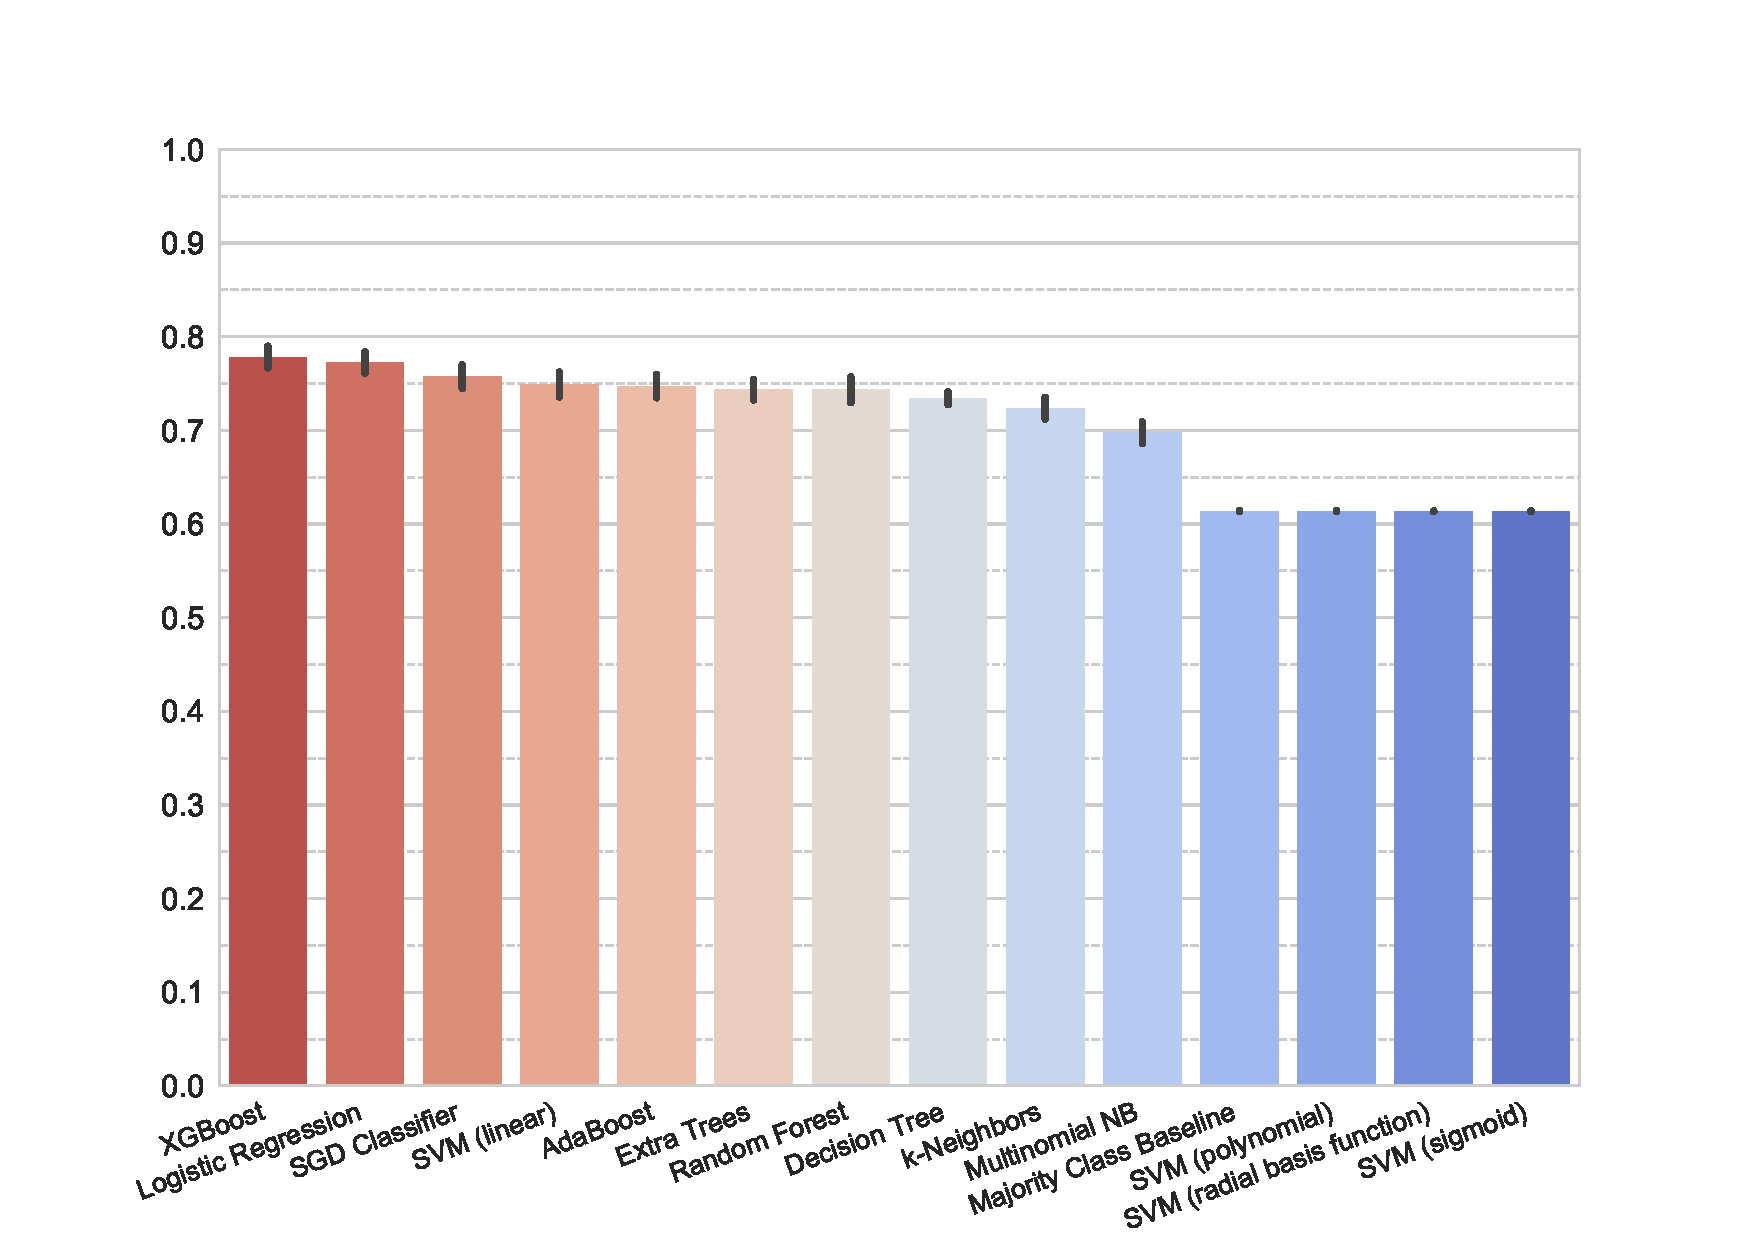
\includegraphics[width=1\linewidth]{images/classifier}
\end{figure}


Tree-based methods and linear models worked well. Support Vector Machines with non-linear kernels assigned \texttt{NONE} to all sentences.

As XGBoost and Logistic Regression achieved high f1 scores, no further investigations on the performance of other algorithms was done. A set of hyper-parameters for XGBoost was tested using exhaustive grid search and randomized search. However, no significant increase in the f1 score could be achieved.

In the following sections, all experiments were conducted using XGBoost with 1000 estimators.


\section{Features}
\label{sec:features}
Several vector representations were tested as features. The simplest one was a binary \emph{bag-of-words} model realised with scikit-learn's \texttt{CountVectorizer}. Another vector representation was generated with the five-hundred most frequent part-of-speech bi-, tri and four-grams (called \emph{POS n-grams}). The \emph{mean word embedding} vector was created by calculating the mean of each word's GloVe vector (as contained in spaCy's \texttt{en\_core\_web\_lg}\footnote{\url{https://spacy.io/models/en\#section-en\_core\_web\_lg}} model). The pretrained \emph{InferSent} model\footnote{\url{https://github.com/facebookresearch/InferSent} (checked 13.05.2018)} was used to create sentence embedding vectors.

A boolean feature capturing the appearance of a comparative adjective (called \emph{Contains JJR}) \footnote{Tag \emph{JJR} in the Penn Treebank (\url{https://www.ling.upenn.edu/courses/Fall\_2003/ling001/penn\_treebank\_pos.html})} was tested as well. Part-of-speech tagging for all features was done with spaCy.\newline

Two preprocessing steps were used to generate the input for the feature calculation.
\begin{table}[ht]
\centering

\caption{Preprocessing examples for the sentence \enquote{\emph{In my mind, Python is better than Ruby}}}
\label{preprocessing_example}
\begin{tabularx}{\linewidth}{llX}
\toprule
Step 1 & Step 2 & Result \\ \midrule
Middle part & untouched & Python is better than Ruby \\
Middle part & removal & is better than \\
Full sentence & distinct replacement &In my mind, OBJECT\_A is better than OBJECT\_B \\
First part & removal & In my mind, \\
\bottomrule
\end{tabularx}

\end{table}

The first preprocessing step decided if the full sentence or a part of it should be used. The \emph{first part} contained all words from the beginning of the sentence to the first object, while the \emph{last part} contained all words from the second object to the end of the sentence. The \emph{middle part} contained all words between the first and the second object.

The second step was done to check the importance of the objects for the classification. The objects either stayed untouched, were removed or replaced. Two different replacement strategies were tested. First, both objects were replaced by the term \mbox{\emph{OBJECT} (\emph{replacement})}. Second, the first object was replaced by \emph{OBJECT\_A} and the second by \emph{OBJECT\_B} (\emph{distinct replacement}). This resulted in sixteen versions of each of the features mentioned above (four parts $\times$ four object strategies). Some examples are shown in Table \ref{preprocessing_example}.\newline


\label{sec:lexnet_feat_desc}
Two features based on LexNet were created to encode dependency parsing information. The original code of LexNet was used to create the string representation of paths, as described in Section \ref{sec:lexnet}. An LSTM was used to create path embeddings out of the string paths. Because the paper does not mention any details about the LSTM encoder, different architectures and hyper-parameter values were tested. The best results were achieved with the architecture described in figure \ref{fig:lexnetnn}.

The addition of more layers or neurons did not increase the performance of the network. This is also true for adding bidirectionality to the LSTM layer. The paths (encoded as one-hot vectors) were used as targets for the network. Keras' embedding layer was used to create word embeddings of length 100 for the string path components.

\begin{figure}[htbp]
\centering
\caption{Architecture of the LSTM path encoder. The embedding layer creates word embeddings for the path edges, which are fed into an LSTM with 200 neurons. The result is pooled (pool size of two) and fed into a softmax layer. Keras \cite{chollet2015keras} was used to implement the network. The network was trained for 150 epochs with a batch size of 128 and RMSprop as the optimizer.}
\label{fig:lexnetnn}
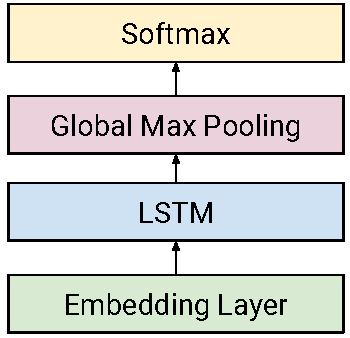
\includegraphics{images/lex_arch}
\end{figure}



Different setups for the string path creation were tested. In the original implementation, the paths were restricted to a length of four. The directionality of edges was restricted as well. The first object must be reachable from the lowest common head of the two objects by following left edges only, the second one by following right edges. In the following, this setup is called \emph{original}. However, only 1519 sentences from the training set got a path with this restrictions. 

To overcome this problem, the restrictions were relaxed. The second LexNet setup (called \emph{customised}) limits the paths to a size of sixteen and abolishes the directionality restriction. With this setup, only 399 sentences do not get a path.\footnote{All sentence without a generated path get the artifical path \emph{NOPATH}. The customised version of LexNet is available at \url{https://github.com/ablx/LexNET}}






\section{Classification Experiments}
\subsection{Baselines}
\label{sec:3_baseline}
As described in Section \ref{sec:argmine}, there is no task which is similar enough to the one at hand which could be used as a baseline. Thus, two baselines were created. 
The first baseline, shown in Table \ref{tbl:3stratifiedbaseline} and \ref{tbl:binmaj}, was created by assigning classes to the data at random, respecting the distribution of classes in the original data.  
% 24.3
\begin{table}[!htb]
	\begin{minipage}{.5\linewidth}
		\caption{Random (stratified) baseline for the three-class scenario.}
		\label{tbl:3stratifiedbaseline}
		\centering
		      
		\begin{tabularx}{0.97\linewidth}{Xrrrr}
			\toprule
			                & precision                    & recall                       & f1 score                     \\ \midrule 
			\texttt{BETTER} & 0.19 \scriptsize{$\pm$0.01} & 0.21 \scriptsize{$\pm$0.01} & 0.20 \scriptsize{$\pm$0.01} \\ 
			\texttt{WORSE}  & 0.06 \scriptsize{$\pm$0.02} & 0.05 \scriptsize{$\pm$0.02} & 0.06 \scriptsize{$\pm$0.03} \\ 
			\texttt{NONE}   & 0.73 \scriptsize{$\pm$0.00}  & 0.73 \scriptsize{$\pm$0.00} & 0.73 \scriptsize{$\pm$0.00} \\ 
			avg.         & 0.57 \scriptsize{$\pm$0.00} & 0.58 \scriptsize{$\pm$0.01} & 0.57 \scriptsize{$\pm$0.00} \\ 
			\bottomrule
		\end{tabularx} 
		
	\end{minipage}%
	\begin{minipage}{.5\linewidth}
		\centering
		\caption{Majority class baseline for the  for the three-class scenario.}
		\label{tbl:3majoritybaseline}
		\begin{tabularx}{0.97\linewidth}{Xrrrr}
			\toprule
			                & precision                    & recall                       & f1 score                                    \\ \midrule 
			\texttt{BETTER} & 0.00 \scriptsize{$\pm$0.00} & 0.00 \scriptsize{$\pm$0.00} & 0.00 \scriptsize{$\pm$0.00}                \\ 
			\texttt{WORSE}  & 0.00 \scriptsize{$\pm$0.00} & 0.00 \scriptsize{$\pm$0.00} & 0.00 \scriptsize{$\pm$0.00}                \\ 
			\texttt{NONE}   & 0.73 \scriptsize{$\pm$0.00}     & 1.00 \scriptsize{$\pm$0.00} & 0.84 \scriptsize{$\pm$0.00}                \\ 
			avg.         & 0.53 \scriptsize{$\pm$0.00} & 0.73 \scriptsize{$\pm$0.00} & \textbf{0.61} \scriptsize{$\pm$0.00} \\ 
			\bottomrule
		\end{tabularx}
	\end{minipage} 
\end{table}


The second baseline predicts all sentences as \texttt{NONE}. The results are shown in tables \ref{tbl:3majoritybaseline} and \ref{tbl:binstrat}.



\begin{table}[!htb]
	\begin{minipage}{.5\linewidth}
		\caption{Random (stratified) baseline for the binary scenario.}
		\label{tbl:binmaj}
		\centering
		      
		\begin{tabularx}{0.97\linewidth}{Xrrrr}
			\toprule
			              & precision                    & recall                       & f1 score                              \\ \midrule 
			\texttt{ARG}  & 0.26 \scriptsize{$\pm$0.03} & 0.26 \scriptsize{$\pm$0.03} & 0.26 \scriptsize{$\pm$0.03}          \\ 
			\texttt{NONE} & 0.72 \scriptsize{$\pm$0.01} & 0.72 \scriptsize{$\pm$0.01} & 0.72 \scriptsize{$\pm$0.01}          \\ 
			avg.       & 0.60 \scriptsize{$\pm$0.02} & 0.60 \scriptsize{$\pm$0.02} & 0.60 \scriptsize{$\pm$0.02} \\ 
			\bottomrule
		\end{tabularx}
		
	\end{minipage}%
	\begin{minipage}{.5\linewidth}
		\centering
		\caption{Majority class baseline for the binary scenario.}
		\label{tbl:binstrat}
		\begin{tabularx}{0.97\linewidth}{Xrrrr}
			\toprule
			              & precision                    & recall                       & f1 score                     \\ \midrule 
			\texttt{ARG}  & 0.00 \scriptsize{$\pm$0.00} & 0.00 \scriptsize{$\pm$0.00} & 0.00 \scriptsize{$\pm$0.00} \\ 
			\texttt{NONE} & 0.73 \scriptsize{$\pm$0.00} & 1.00 \scriptsize{$\pm$0.00} & 0.84 \scriptsize{$\pm$0.00} \\ 
			avg.       & 0.53 \scriptsize{$\pm$0.00} & 0.73 \scriptsize{$\pm$0.00} & \textbf{0.61} \scriptsize{$\pm$0.00} \\ 
			\bottomrule
		\end{tabularx}
	\end{minipage} 
\end{table}
Scikit-learns \texttt{DummyClassifer} was used for all baselines.

\subsection{Results}
\label{sec:3_results}
The classification results of the best performing feature configurations in the three-class scenario are presented in figures \ref{fig:3_f1} (f1 score), \ref{fig:3_precision} (precision) and \ref{fig:3_recall} (recall). Each feature was tested and evaluated using five stratified folds. The black bar shows the standard derivation. All scores were calculated with scikit-learn's metric module. All features except the \emph{LexNet (original)} features used the middle part of the sentence and left the objects untouched. In the LexNet features, the objects were replaced with \emph{Objecta} and \emph{Objectb}. \emph{LexNet (original)} used the full sentence.

% 15.5
\begin{figure}[htbp]
      \caption{\textbf{F1 score} for the three-class scenario using XGBoost. The grey bar shows the weighted average. The feature names (see Section \ref{sec:features}) are presented on the x-axis, the f1 score on the y-axis. The black bar shows the standard derivation.} 
    \label{fig:3_f1}
 \centering
	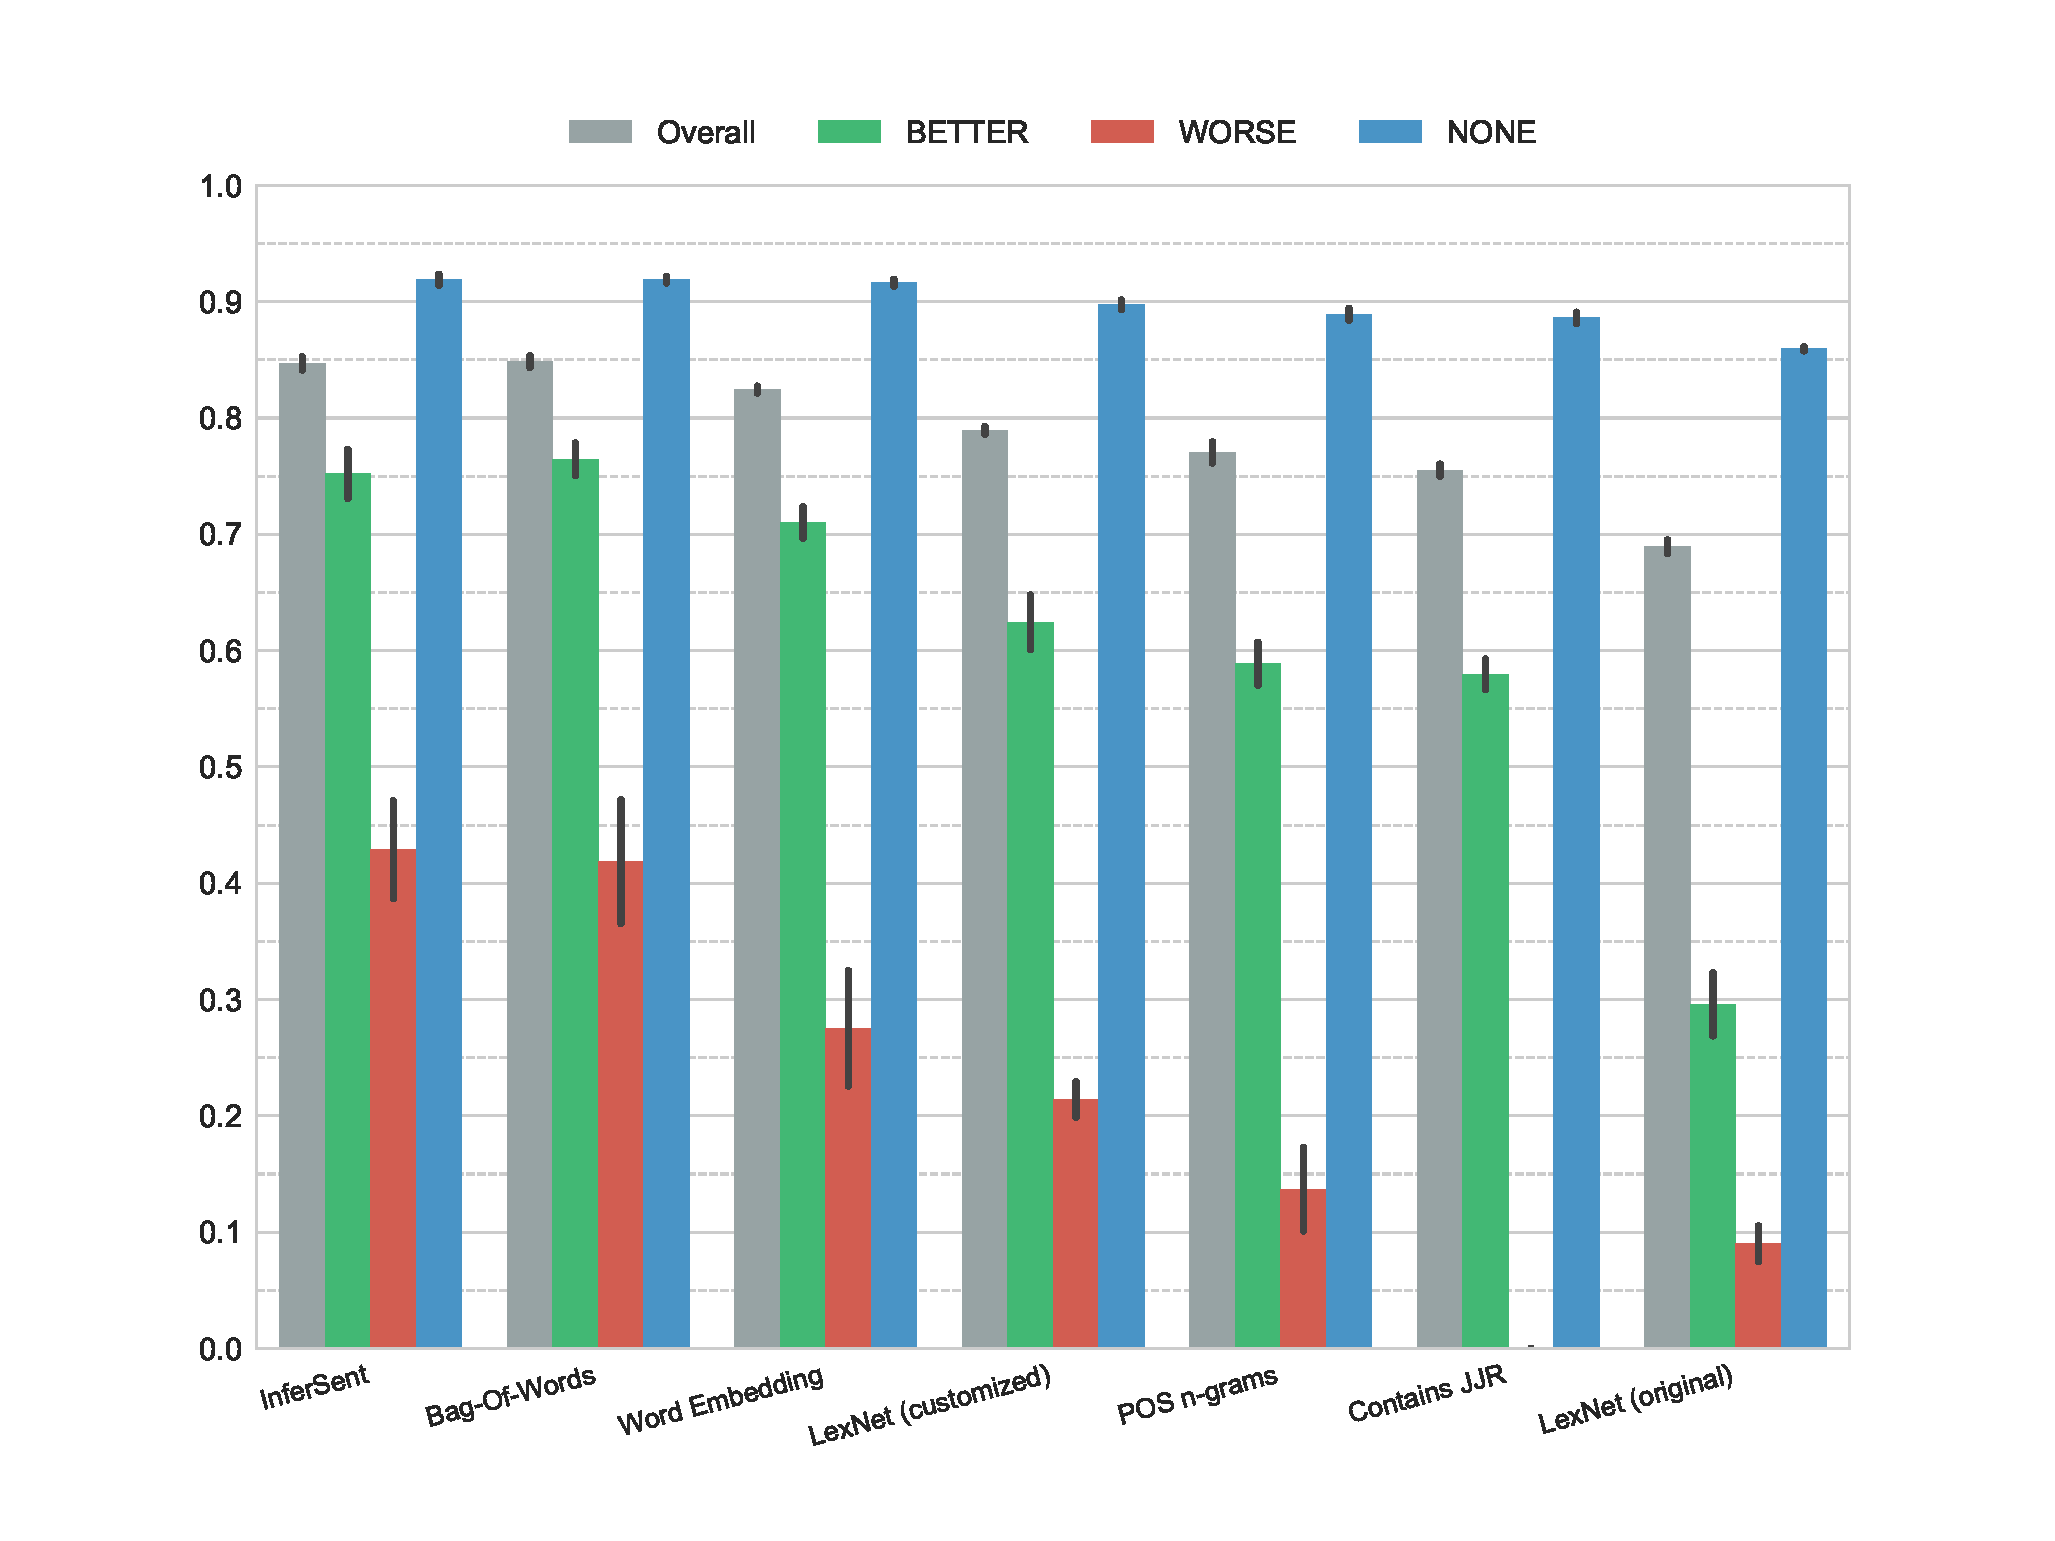
\includegraphics[width=0.9\textwidth]{images/experiments/f1-False}

\end{figure}


% 15.5 f1 scores
The best feature (bag-of-words) yielded a score 24 points above the baseline. The worst feature (\emph{LexNet (original)}) was still eight points above the baseline. Bag-of-words (f1 score 0.848) and InferSent (f1 score 0.842) delivered almost identical results. The boolean feature that captures comparative adjectives in the middle of the sentence yielded a f1 score over the baseline as well. However, it did not assign any examples to the class \texttt{WORSE}.
% 15.5 lexnet dinge

Despite the fact that only 1519 sentences got a path embedding for \emph{LexNet (original)}, the feature is able to predict some sentences correctly. This indicates that this feature setup is reasonable and would work probably work well if more examples were present. An experiment with only the 1519 sentences confirms this, as the feature is then able to achieve an f1 score of 0.75.

\begin{figure}[p]
         \caption{\textbf{Precision} for the three-class scenario using XGBoost. The grey bar shows the weighted average. The feature names (see Section \ref{sec:features}) are presented on the x-axis, the precision score on the y-axis. The black bar displays the standard derivation.} 
    \label{fig:3_precision}
 \centering
	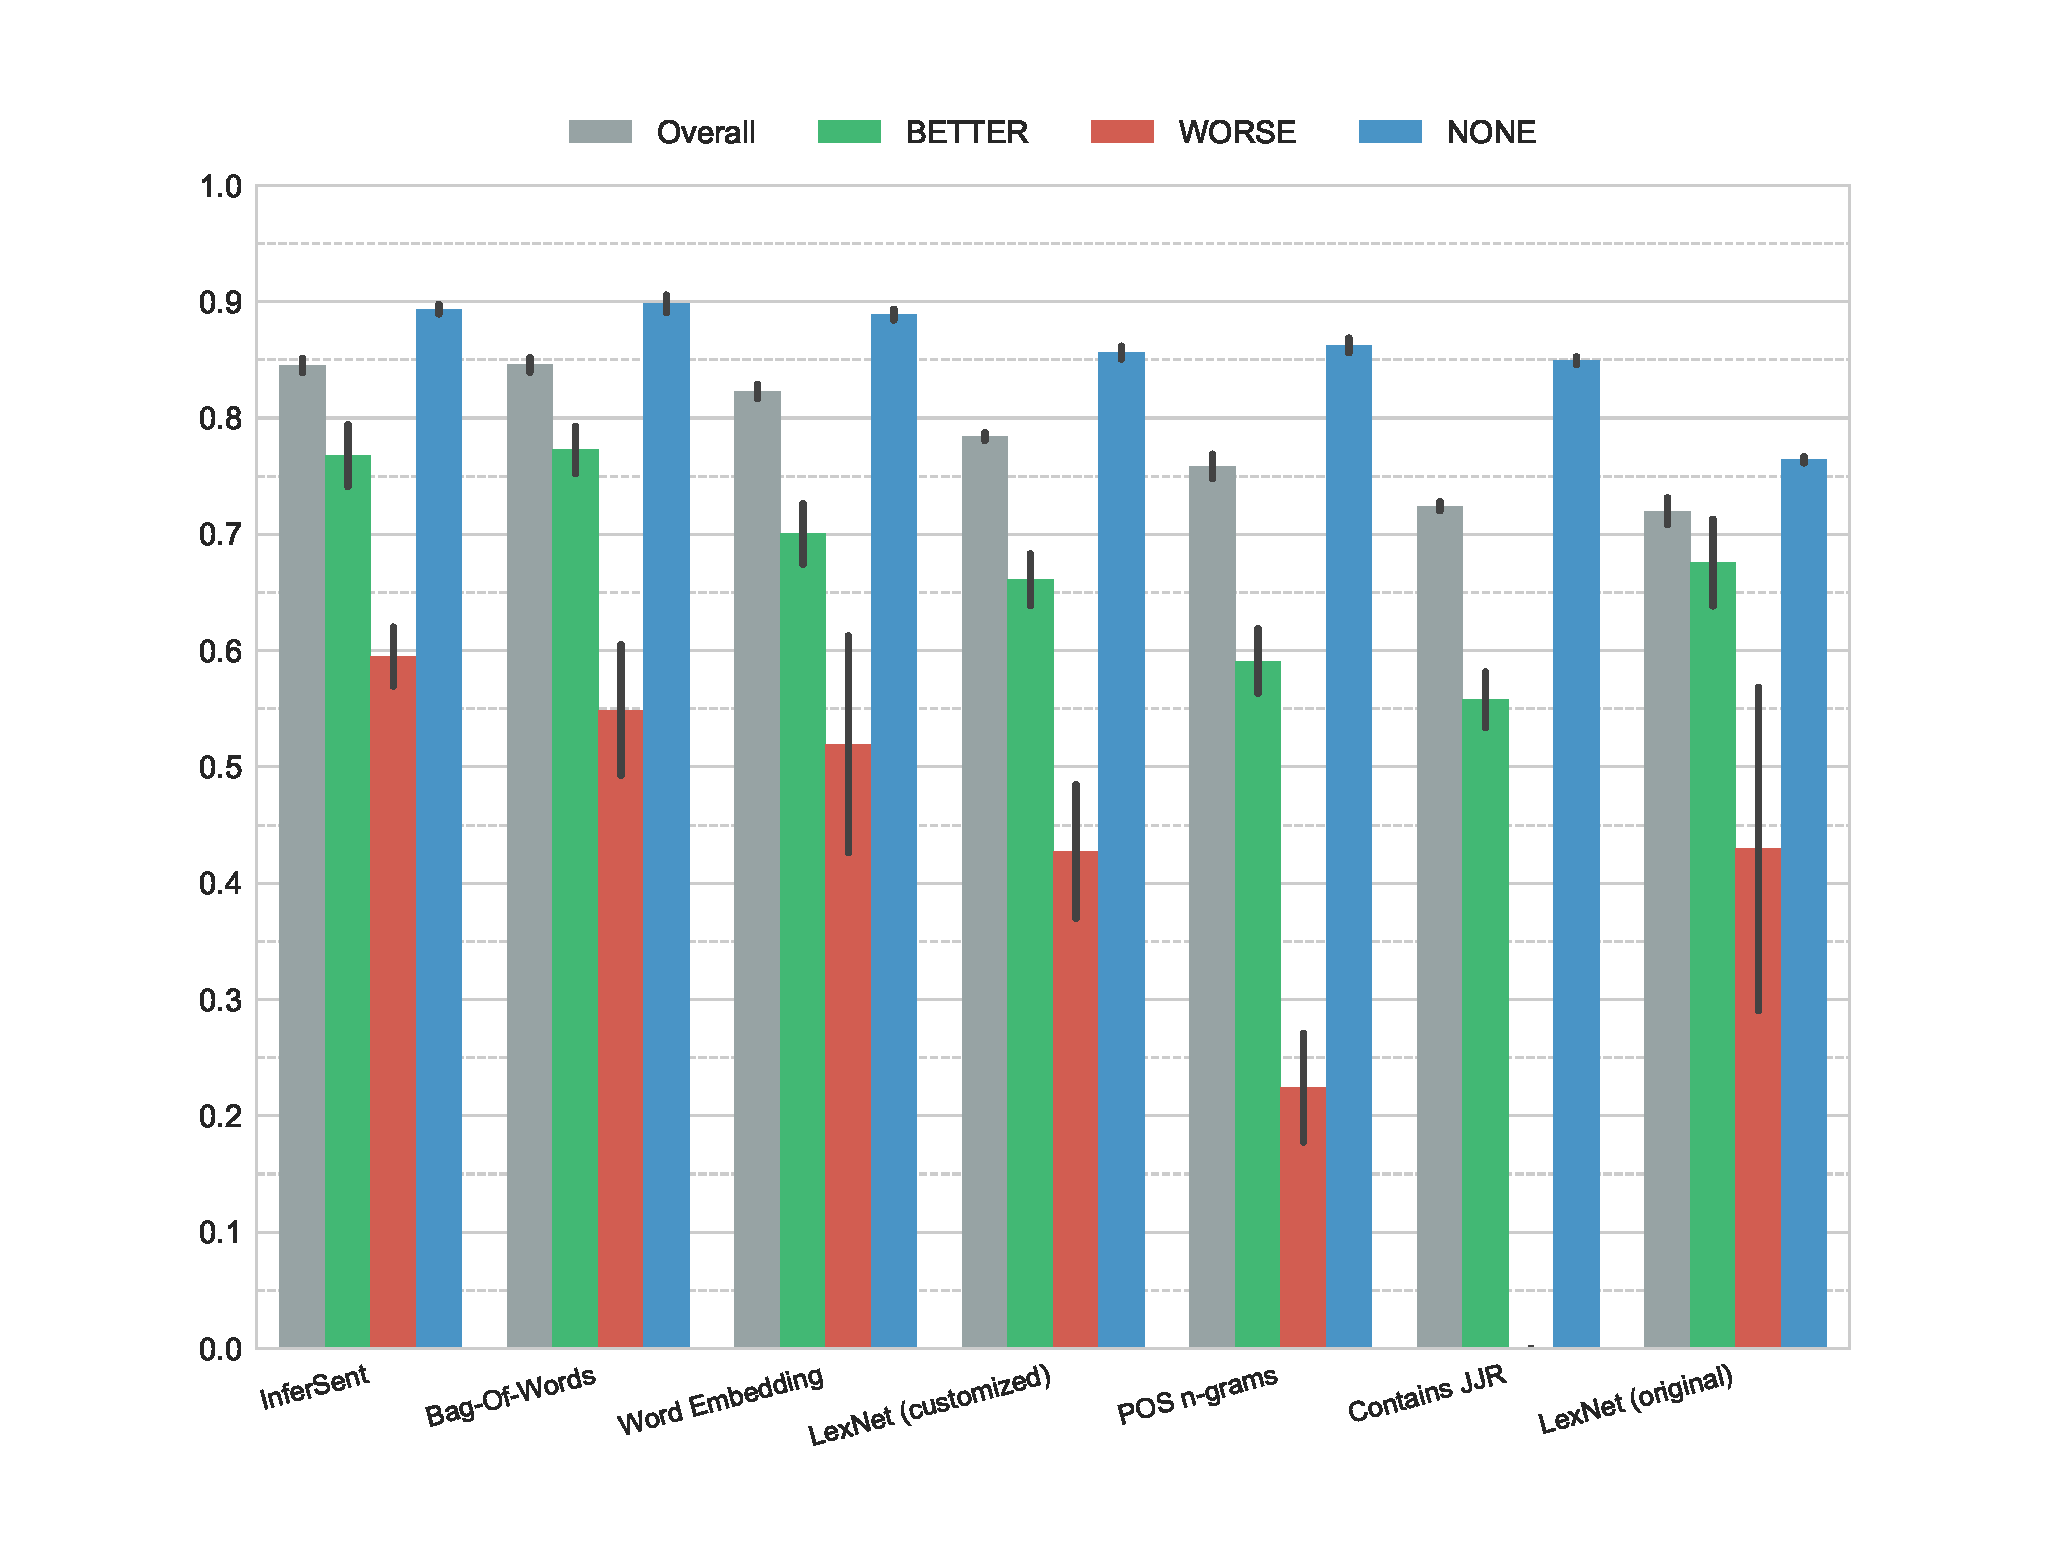
\includegraphics[width=0.9\textwidth]{images/experiments/precision-False}
\end{figure}

  \begin{figure}[p]
              \caption{\textbf{Recall} for the three-class scenario using XGBoost. The grey bar shows the weighted average. The feature names (see Section \ref{sec:features}) are presented on the x-axis, the recall score on the y-axis. The black bar shows the standard derivation.} 
       \label{fig:3_recall}
 \centering
	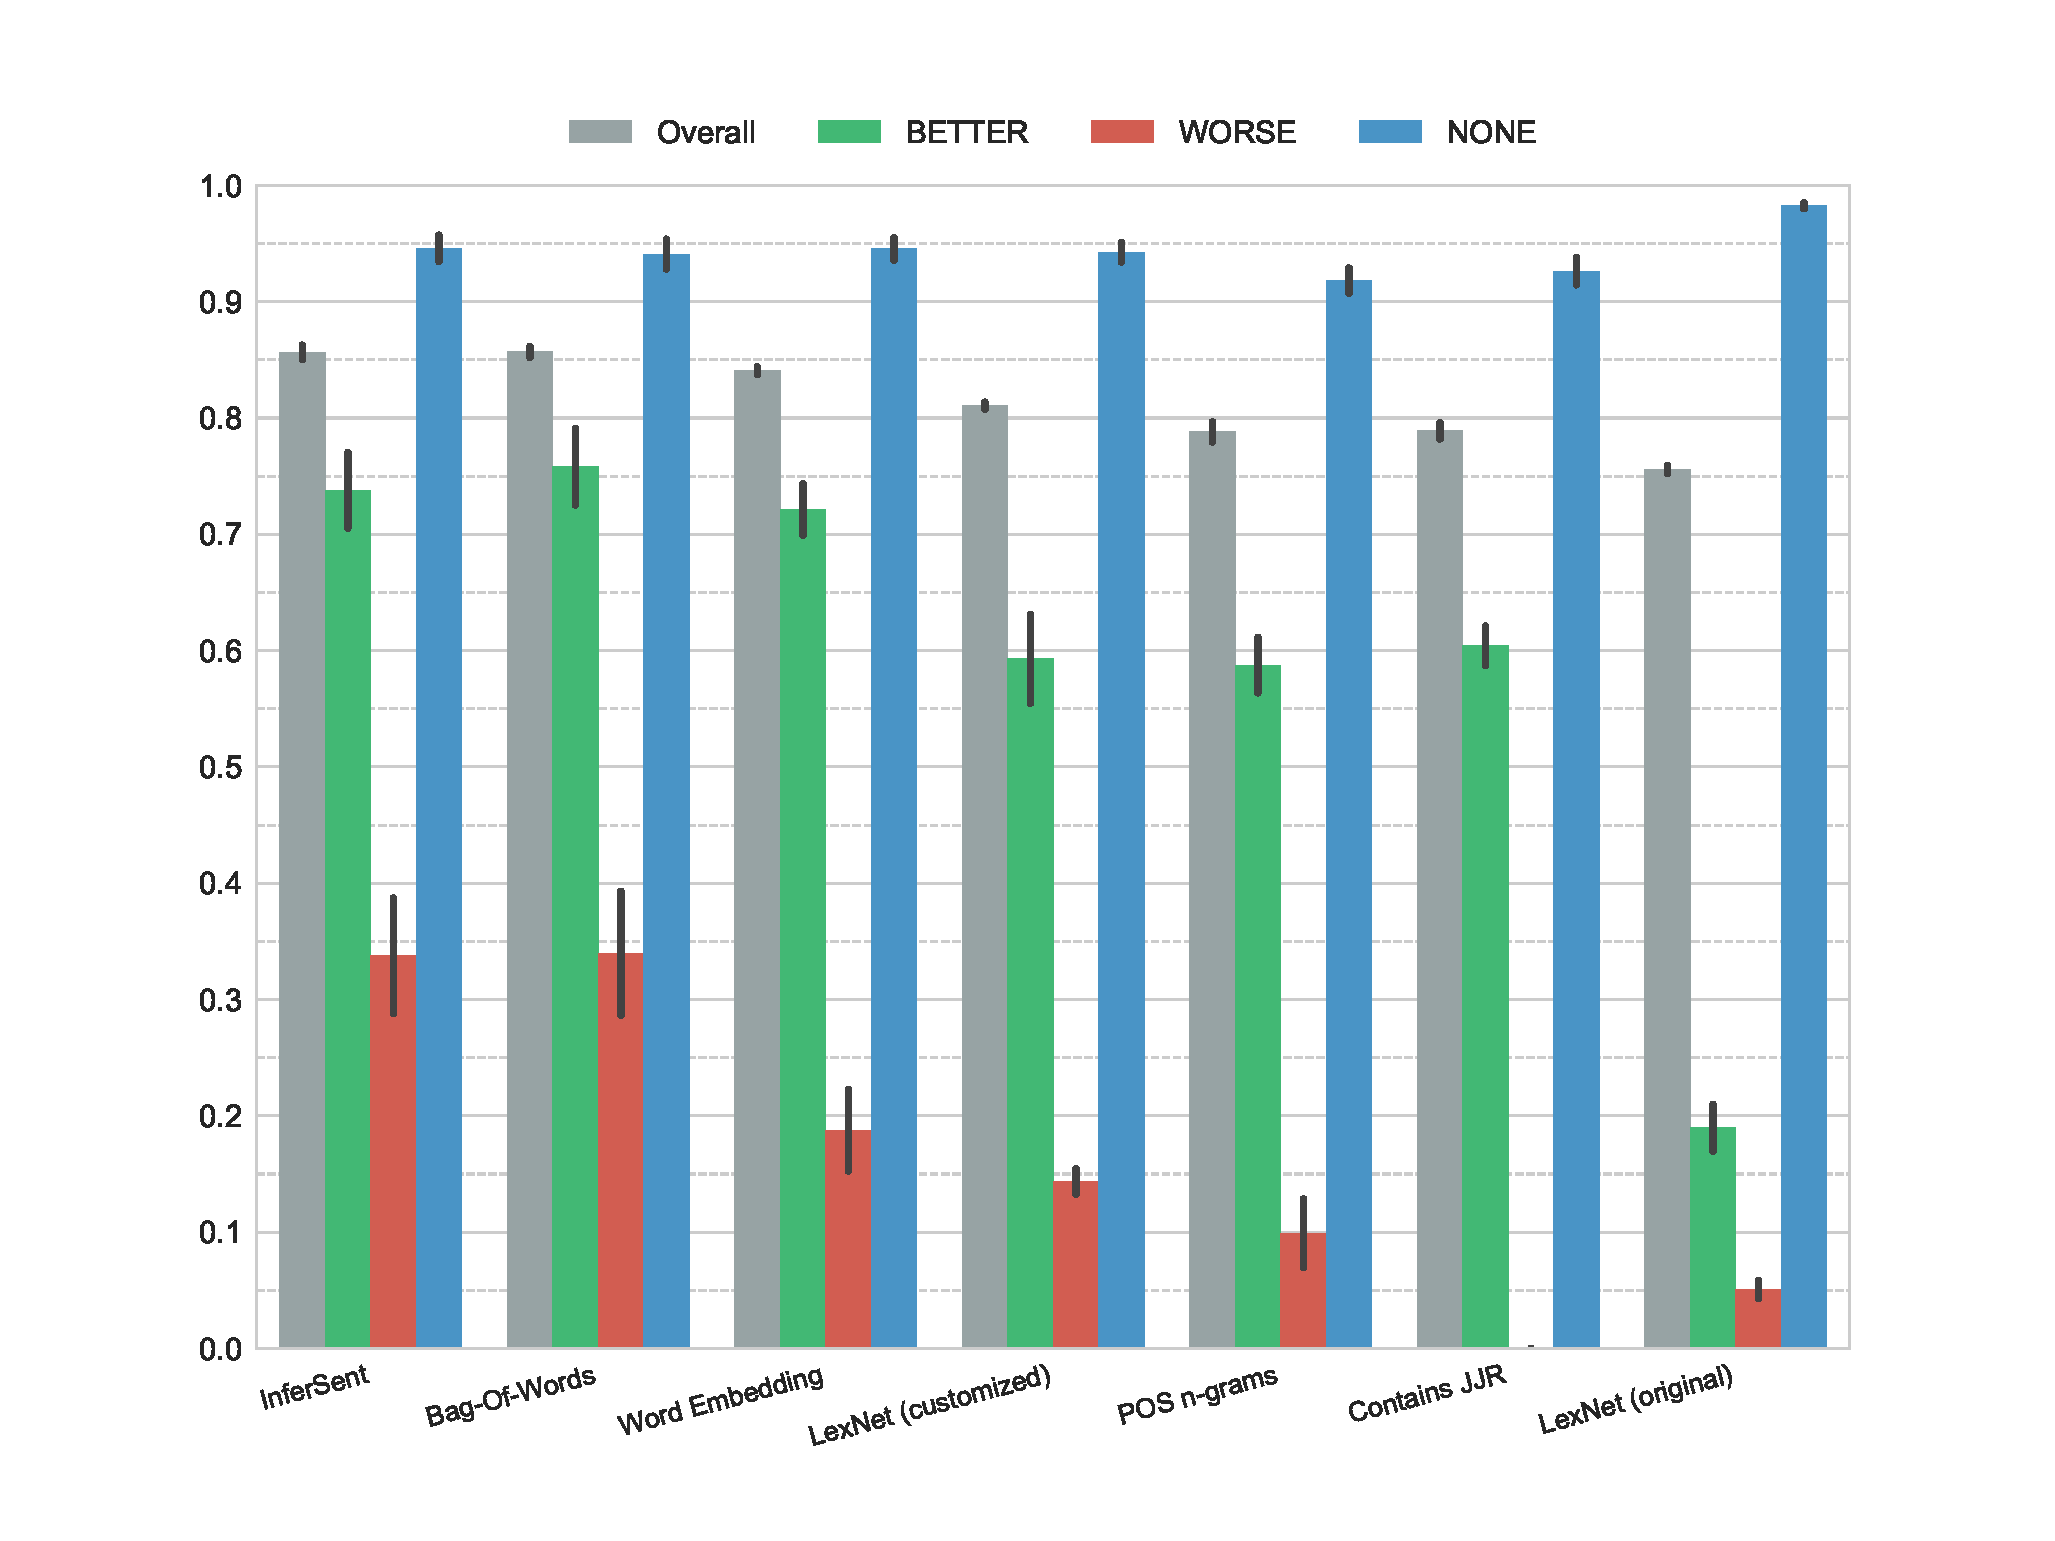
\includegraphics[width=0.9\textwidth]{images/experiments/recall-False}
\end{figure}

\FloatBarrier

% === binary 
Figures \ref{fig:2_f1} (f1 score), \ref{fig:2_precision} (precision) and \ref{fig:2_recall} (recall) show the results for the binary classification.
\begin{figure}[htbp]
      \caption{\textbf{F1 score} for the binary scenario using XGBoost. The grey bar shows the weighted average. The feature names (see Section \ref{sec:features}) are presented on the x-axis, the f1 score on the y-axis. The black bar displays the shows derivation.} 
 
% 15.5
    \label{fig:2_f1}
 \centering
	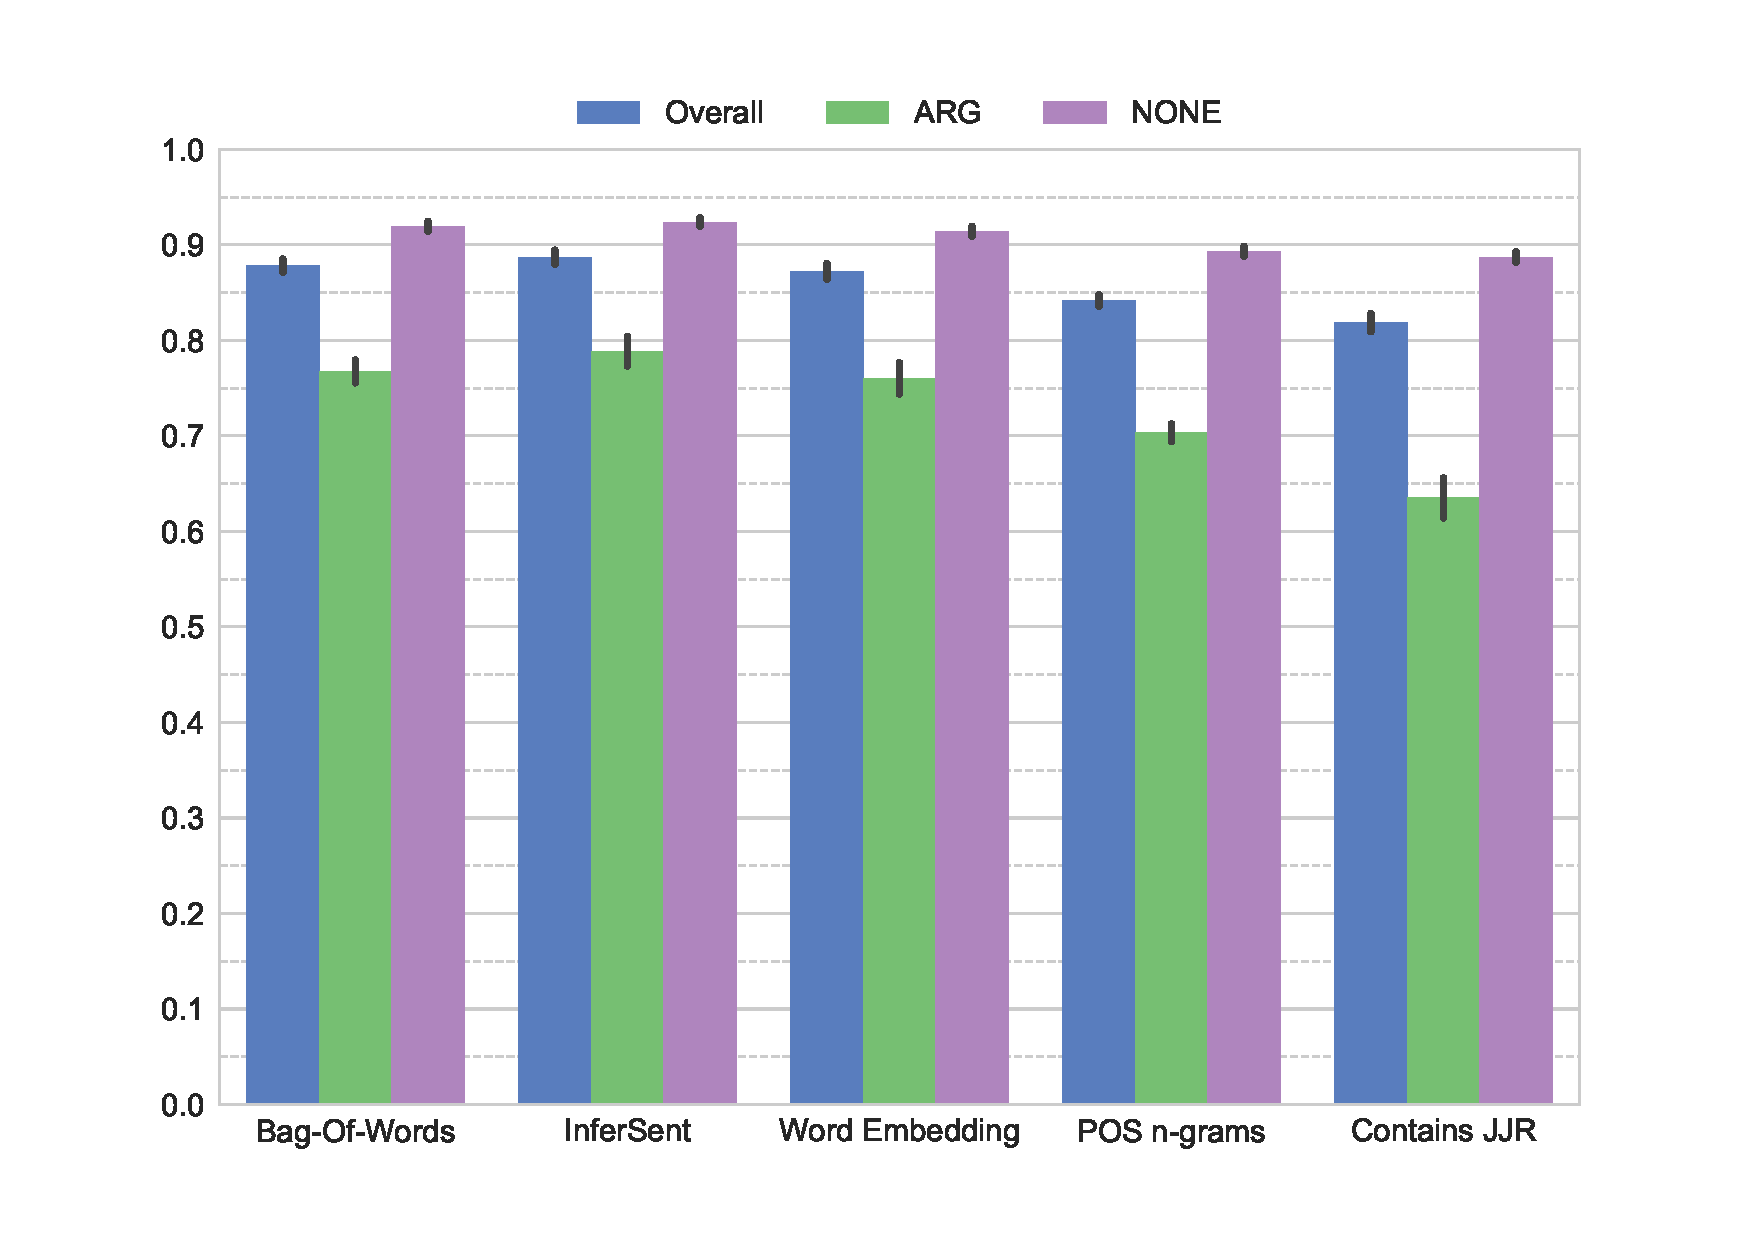
\includegraphics[width=1\textwidth]{images/experiments/f1-True}

\end{figure}
As with the three-class scenario, InferSent (f1 score 0.886) and the bag-of-words (f1 score 0.882) performed best and got almost equal results. They are closely followed by mean word embeddings. In summary, all vector representations worked good and got similar f1 scores. The feature \emph{LexNet (original)} is again the worst, yet the score is ten points above the baseline.% 15.5






% 15.5
\begin{figure}[p]
         \caption{\textbf{Precision} for the binary scenario using XGBoost. The grey bar shows the weighted average. The feature names (see Section \ref{sec:features}) are presented on the x-axis, the precision score on the y-axis. The black bar displays the standard derivation.} 
    \label{fig:2_precision}
    \centering
	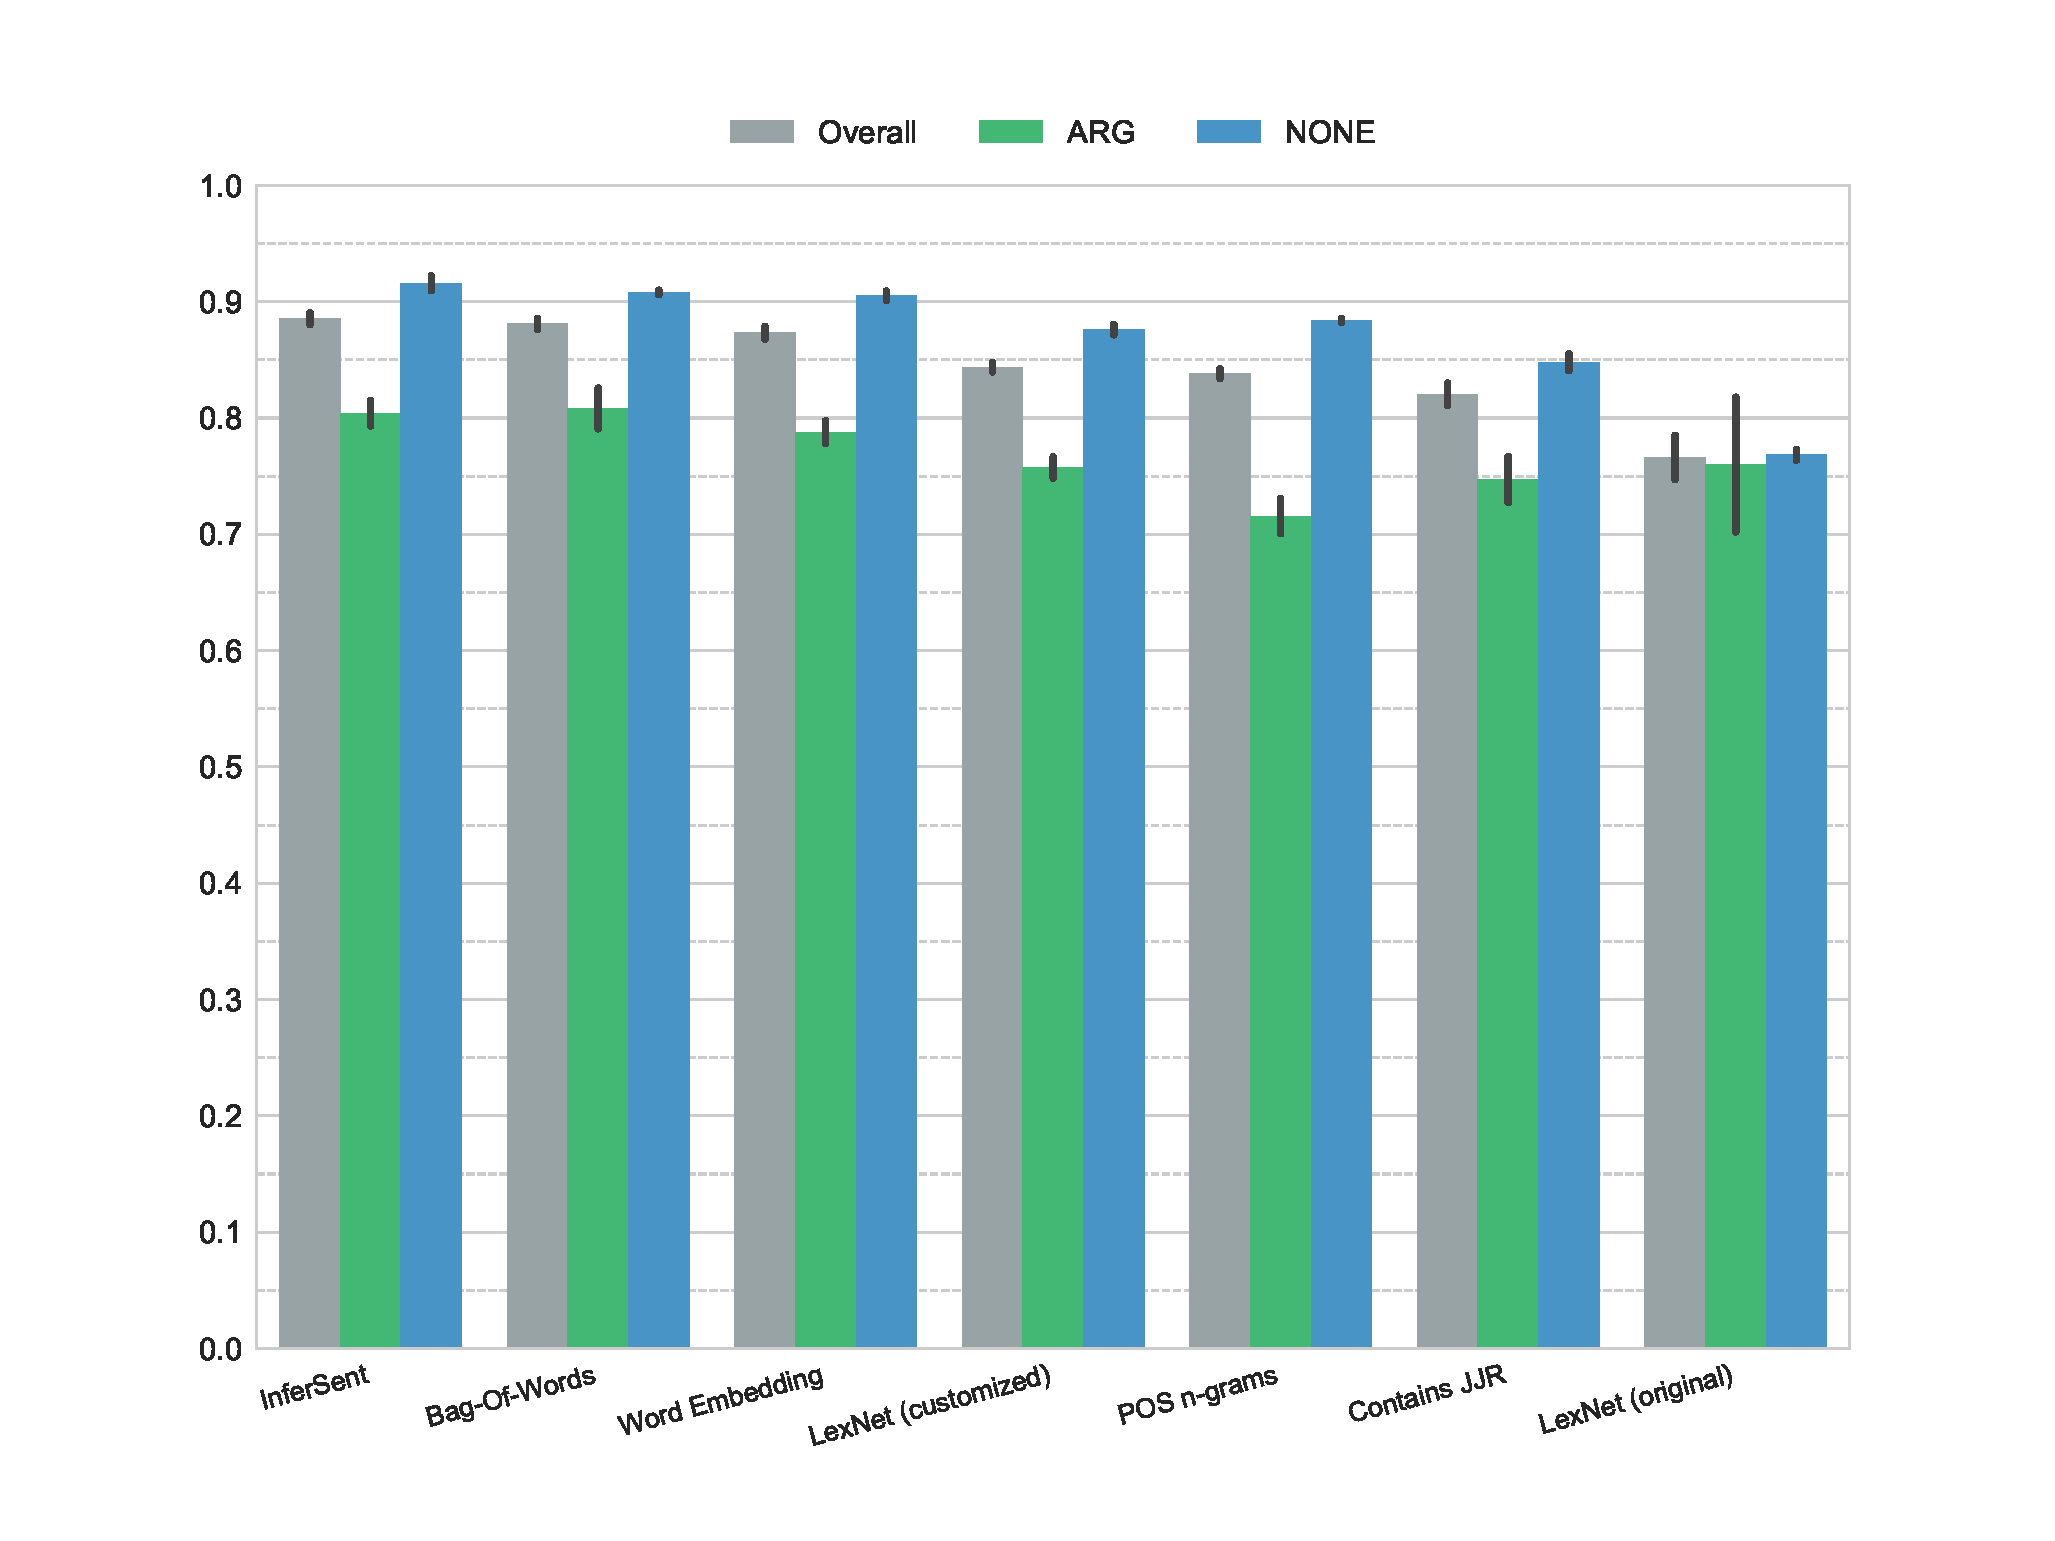
\includegraphics[width=0.9\linewidth]{images/experiments/precision-True}
    \end{figure}
    % 15.5
    \begin{figure}[p]
              \caption{\textbf{Recall} for the binary scenario using XGBoost. The grey bar shows the weighted. The feature names (see Section \ref{sec:features}) are presented on the x-axis, the binary score on the y-axis. The black bar displays the standard derivation.} 
       \label{fig:2_recall}
 \centering
	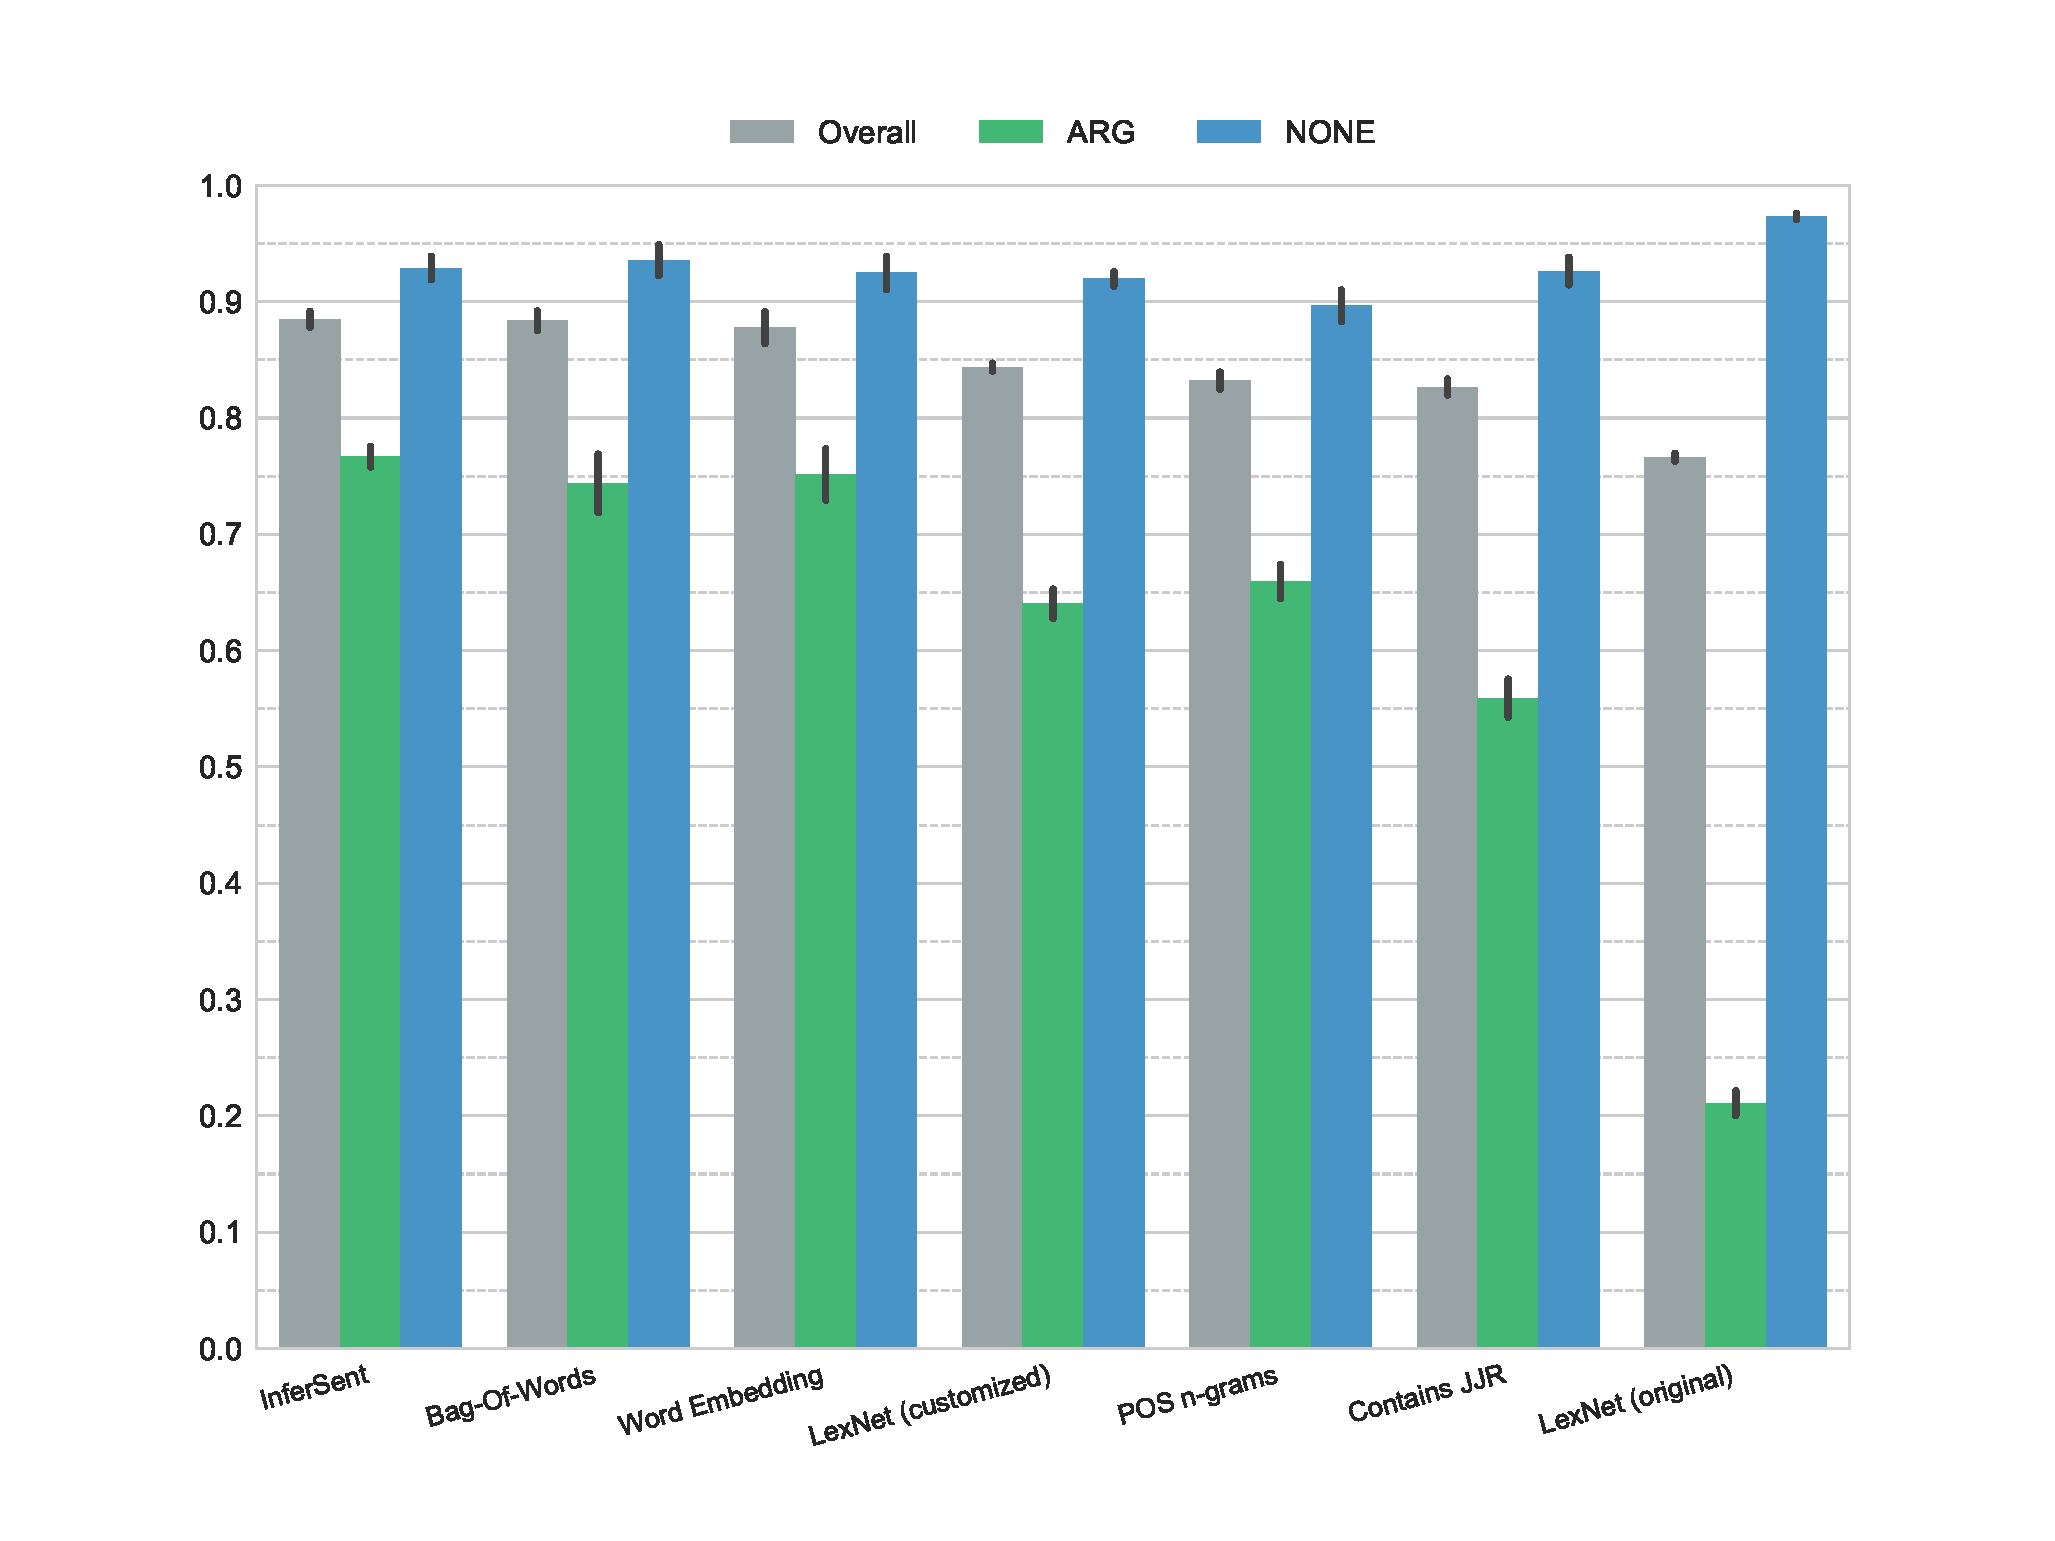
\includegraphics[width=0.9\linewidth]{images/experiments/recall-True}

\end{figure}



\FloatBarrier
\subsection{Error analysis}
\label{sec:error_analysis}
Figure \ref{fig:3_conf_inf} displays the confusion matrix for the best lexical feature in the three-class scenario (InferSent, also the best feature overall), while figure \ref{fig:3_conf_uni} shows the confusion matrix for the best syntax feature (customised LexNet).
 The confusion matrices of each fold per feature were summed up to create the figures.



% 15.5
\begin{figure}[h]
    \begin{minipage}{.5\linewidth}
   \caption{Confusion matrix for the InferSent feature using XGBoost in the three-class scenario.} 
    \label{fig:3_conf_inf}
 \centering
	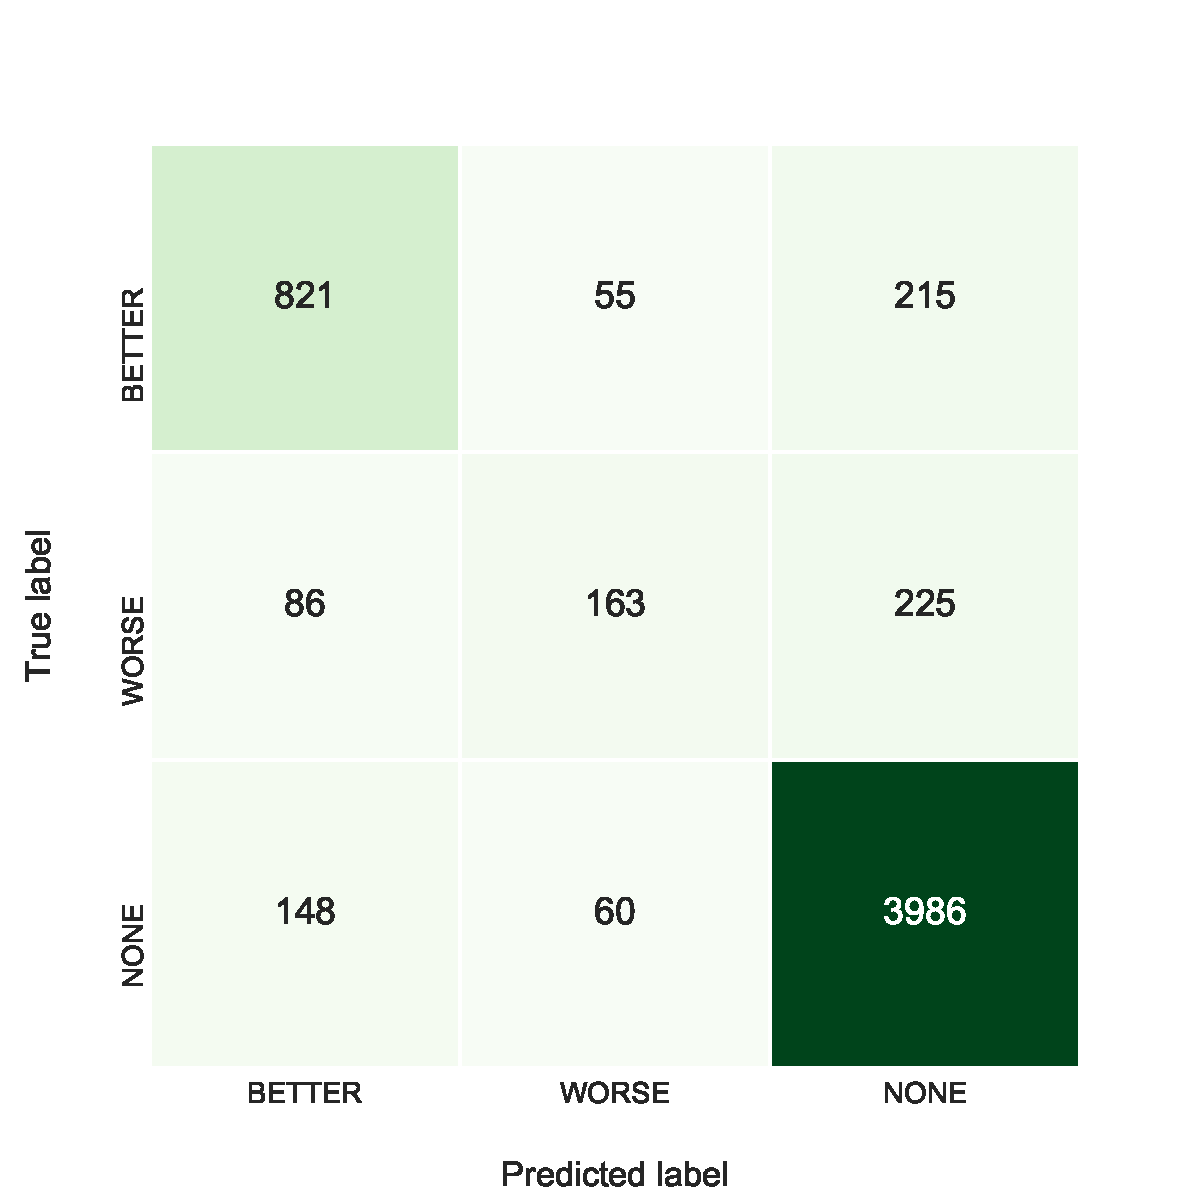
\includegraphics[width=1\linewidth]{images/experiments/conf-InferSent_False}
  \end{minipage} \hfill
    \begin{minipage}{.5\linewidth}
  
     \caption{Confusion matrix for the customised LexNet feature using XGBoost in the three-class scenario.} 
       \label{fig:3_conf_uni}
 \centering
	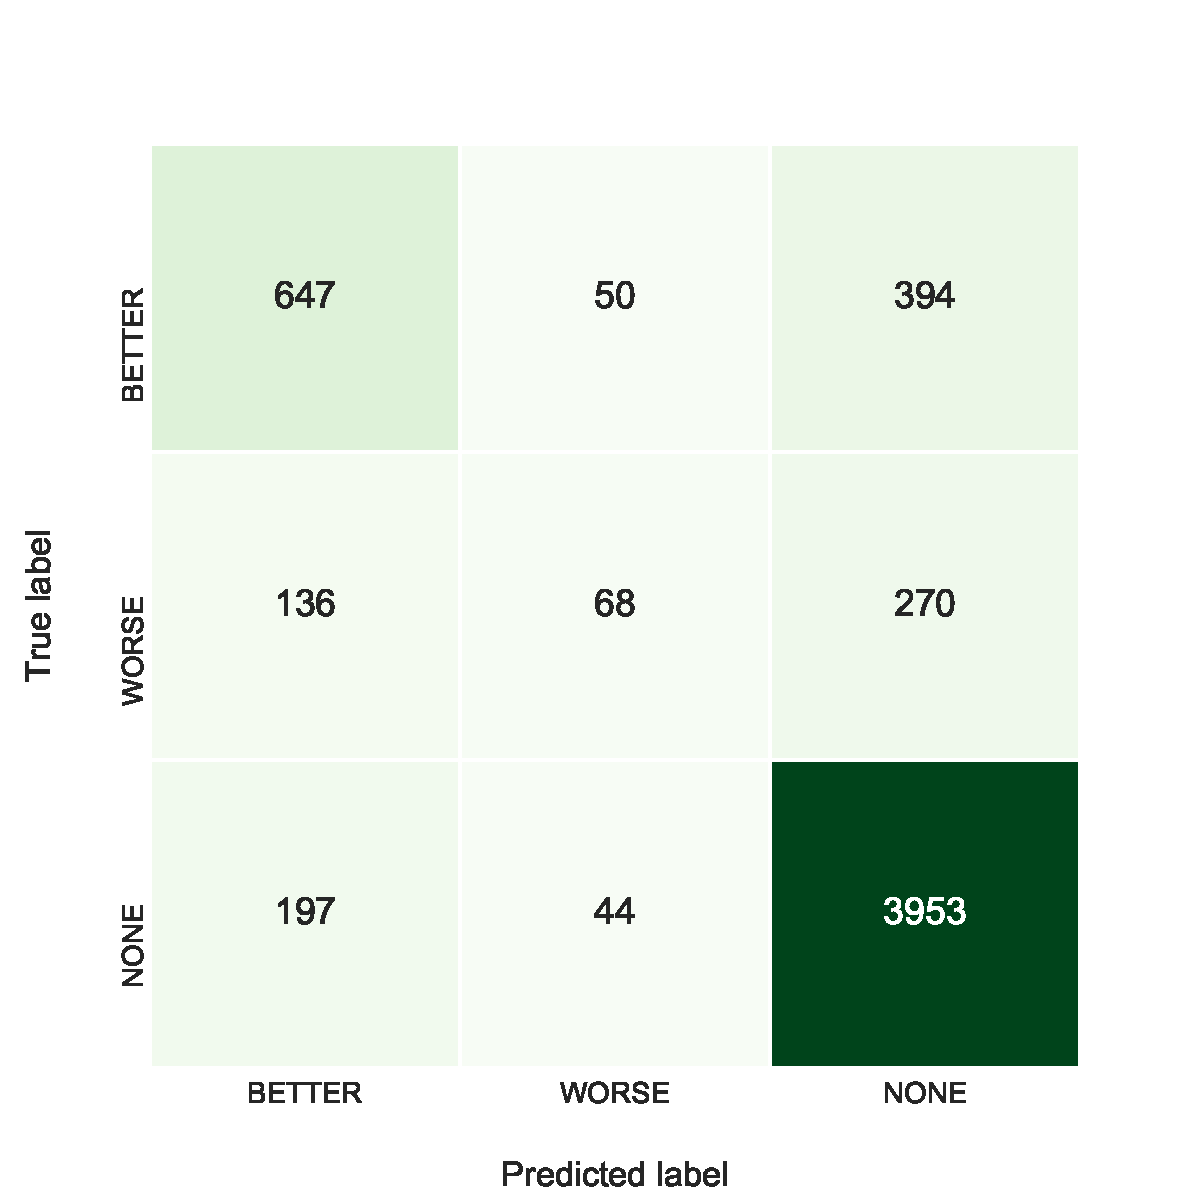
\includegraphics[width=1\linewidth]{images/experiments/conf-middle_paths_unrestricted_16_False}
    \end{minipage} 
\end{figure}

As presented above, \texttt{WORSE} was the hardest class to recognize. The matrices show that it was more often confused with \texttt{NONE} than with \texttt{BETTER}. This is contrary to the expectations. The classes  \texttt{BETTER} and \texttt{WORSE} are representing argumentative sentence. It was expected that the distinction between argumentative and not-argumentative is clearer. 
% 15.55
In total, 1311 sentences were incorrectly classified. Both features made the same errors on 607 sentences. The InferSent feature made 220 additional errors, while the LexNet feature made 484. Surprisingly, the majority of errors was made on sentences with a high confidence. Four-hundred-twenty-five of the shared errors were made on sentences with a confidence of one. InferSent made 156 errors on highly confident sentences, while LexNet made 356. Examples on errors made solely by the InferSent feature are given in Table \ref{tbl:3_mistakes_se}.
\begin{table}[h]
\caption{Example sentences for errors made by XGBoost in the three-class scenario with the InferSent feature. The objects of interest are printed \textbf{bold}. Confidence shows the confidence of the annotators and is calculated as \emph{judgments for majority class / total judgments}.}
\label{tbl:3_mistakes_se}
\begin{tabularx}{\linewidth}{lXrrr}
\toprule
 & Sentence & Predicted & Gold & Confidence \\ \midrule
1& Is \textbf{Python} better than \textbf{Perl}? & \texttt{BETTER} & \texttt{NONE} & 0.6\\ % 15.5

2& Is \textbf{Microsoft} better because of \textbf{Apple}? & \texttt{BETTER} & \texttt{NONE} & 1.0\\ % 15.5
 
3& \textbf{Microsoft} is the devil but \textbf{Sony} truly isn't any better. & \texttt{WORSE} & \texttt{NONE} & 1.0\\ % 15.5

4& \textbf{Python} is much better suited as a "glue" language, while \textbf{Java} is better characterized as a low-level implementation language. & \texttt{BETTER} & \texttt{NONE} & 1.0\\ % 15.5
 
5& Its Azure PaaS/IaaS platform hasn't overtaken \textbf{Amazon} yet in market share, but \textbf{Microsoft} has enjoyed nine straight quarters of growth at 10 percent or better & \texttt{NONE} & \texttt{WORSE} & 1.0\\ % 15.5
 
 6& arrrggghh...\textbf{Python} is a terrible language - only \textbg{Perl} sucks worse. & \texttt{WORSE} & \texttt{BETTER} & 1.0\\ % 15.5
 
7&  Good to see again a \textbf{Renault} ahead of a \textbf{Ferrari}. & \texttt{NONE} & \texttt{BETTER} & 1.0\\ % 15.5
\bottomrule
\end{tabularx}
\end{table}
% 15.5
The first two sentences look comparative, but they are questions. As stated in the guidelines, all questions should be labelled as \texttt{NONE}, but InferSent frequently classified questions as comparative. Sentences three and four are comparative, but it has no clear winner of the comparison. The guidelines formulated that only sentences with clear winners should be labelled with \texttt{BETTER} or \texttt{WORSE}. InferSent was not able to learn this restriction. Sentence six has three negative words in it. Sentence seven is hard to classify, as it does not contain any cue word.
% 15.5

Table \ref{tbl:3_mistakes_lexnet} shows examples for errors exclusively made by the LexNet feature. As described in Section \ref{sec:lexnet_feat_desc}, 399 of the sentences did not get a dependency path. However, only 36 of the wrongly classified sentences did not had a path.

It is salient that the LexNet feature maked errors an fairly simple sentences like the first one in Table \ref{tbl:3_mistakes_lexnet}. While InferSent's errors can be coarsely grouped, the errors made by LexNet seem more random. It is assumed that the amount of training data for the neural network encoder is not big enough to create expressive embeddings. However, the overall result of LexNet indicates that a encoder trained on more data will likely yield good results.

% 15.5
Sentences which were wrongly classified by both features are presented in Table \ref{tbl:3_mistakes_both}. Both features predicted the same class for 477 of the 607 shared errors.

The shared errors are similar to the errors made exclusively by InferSent. Again, they can be coarsely grouped, for instance into questions (sentence one in Table \ref{tbl:3_mistakes_both}) or sentences without a clear winner (sentence four).\newline

In the binary scenario, 1183 errors were made. Both features made the same errors on 380 sentences. LexNet made 520 unique errors, while InferSent made 283. However, 739 errors were already made in the three-class scenario, only 444 errors are new. All in all, the analysis of the errors made in the binary scenario did not gave any new insights. Again, the majority of errors was made on sentences with a high confidence. The errors made exclusively by LexNet seem random again, while the shared errors and the errors made by InferSent have similar sources (e.g. questions, no clear winner, complex sentences). %15.5

\begin{table}[htbp]
\caption{Example errors made by the classifier in the three-class scenario with the LexNet feature. The objects of interest are printed \textbf{bold}. Confidence shows the confidence of the annotators and is calculated as \emph{judgments for majority class / total judgments}.}
\label{tbl:3_mistakes_lexnet}
\begin{tabularx}{\linewidth}{lXrrr}
\toprule
 & Sentence & Predicted & Gold & Confidence \\ \midrule
1 & Right now \textbf{Apple} is worse then \textbf{Microsoft} ever was. & \texttt{BETTER} & \texttt{WORSE} & 0.8 \\ % 15.5

2 & \textbf{california} is a much harder place to practice law than is South \textbf{carolina}. & \texttt{NONE} & \texttt{WORSE} & 1.0\\ % 15.5

3 & \textbf{google+} starts out far faster than \textbf{facebook}, Twitter& \texttt{NONE} & \texttt{BETTER} & 1.0\\ % 15.5

4 & In FPGAs, \textbf{Integer} or fixed-point math can often run 10 to 100 times faster than \textbf{Floating-point} 
computations. & \texttt{NONE} & \texttt{BETTER} & 1.0\\ % 15.5

5 & Your \textbf{iphone} is a much better display than your desktop/\textbf{laptop} & \texttt{NONE} & \texttt{BETTER} & 0.8\\
 \bottomrule
\end{tabularx}
\end{table}

\begin{table}[htbp]
\caption{Example errors made by InferSent and LexNet in the three-label scenario. The objects of interest are printed \textbf{bold}. \emph{Pred. IF} shows the predicted class of the InferSent feature, \emph{Pred. LexNet} the prediction of the LexNet feature. Confidence shows the confidence of the annotators and is calculated as \emph{judgments for majority class / total judgments}.}
\label{tbl:3_mistakes_both}
\begin{tabularx}{\linewidth}{lXrrrr}
\toprule
 & Sentence & Pred. IF & Pred. LexNet & Gold & Conf. \\ \midrule
1 & Is a \textbf{BMW} 3 series \$15,000 better than a \textbf{Ford} Focus? & \texttt{BETTER} & \texttt{BETTER} & \texttt{NONE} & 1.0\\ % 15.5

2 & \textbf{Google} is the main player now, \textbf{Microsoft} are just plain inferior in Mobile & \texttt{NONE} & \texttt{NONE} & \texttt{BETTER} & 1.0\\ % 15.5

3 & Yeah, Nvidia's \textbf{OpenCL} is not good and \textbf{CUDA} is way better. & \texttt{NONE} & \texttt{BETTER} & \texttt{WORSE} & 1.0\\ % 15.5

4 & \textbf{Python} grew out of the need for a "better" \textbf{Perl}. & \texttt{WORSE} & \texttt{NONE} & \texttt{BETTER} & 1.0\\

5 & \textbf{Groovy} code often looks and feels like \textbf{Java} code, but is almost always simpler and easier to use. & \texttt{NONE} & \texttt{NONE} & \texttt{BETTER} & 0.4\\ % 15.5

 \bottomrule
\end{tabularx}
\end{table}


\subsection{Discussion}
Section \ref{sec:3_results} only shows the results for the best performing configuration of each feature. This is, for all cases, the middle part of the sentence. Sentences which are not formed after this pattern caused wrong predictions, as presented \ref{sec:error_analysis}.

Using the full sentence worked second best. Adding the first and/or last part of the sentence did not increase the f1 score at all, no matter if the same or another representation type than the one for the middle part is used. The first and second part alone never got an f1 score above the baseline.

Replacing or removing the objects did not increase the score significantly. In most cases, the difference in the f1 score between no replacement/removal and the best replacement/removal strategy was only reflected in the third or fourth decimal place. Hence, the concrete objects are not important at all for the classification. This is also supported by the fact that adding the word vectors of the objects as features did not increase the result for any feature.

An interesting observation is that the simple bag-of-words model performs equal or better than the more complex models. The simple feature \emph{Contains JJR} (which is only one boolean value) is able to distinguish argumentative and non-argumentative sentences in a pleasing way, yielding an f1 score fourteen points above the baseline.

The values for LexNet path embeddings show that this is a reasonable way to encode sentences. The original setup found only paths for 26\% of the sentences, yet it yielded an f1 score eight points above the baseline. The customisation made it even more powerful. No combination of vector representations increased the score in any way. It was expected that a combination of LexNet features and one of the other features like InferSent will increase the f1 score, as they encode different information (lexical and syntactial). However, this was not the case. Appending the LexNet vectors to the InferSent vectors reduced the scores.

As expected, the smallest class in the data set caused the biggest problems. Precision, recall and f1 score of \texttt{WORSE} have a high standard derivation for most features. Looking at the confusion matrices in figure \ref{fig:3_conf_inf} and \ref{fig:3_conf_uni}, \texttt{WORSE} was confused with \texttt{NONE} for the majority of cases. Intuitively, a confusion between \texttt{WORSE} and \texttt{BETTER} was expected, since both classes should reflect special argumentative sentences in general.

Another interesting observation is that the three-class scenario and the binary scenario made mistakes on the same sentences. In fact, the majority of mistakes made by the binary scenario were made by the three-classes scenario as well.


\section{Evaluation with the held-out data}
\subsection{Results}
\label{sec:final}

The held-out data set contains 1441 sentences (1048 \texttt{NONE}, 273 \texttt{BETTER}, 119 \texttt{WORSE}). The classifier was trained on the complete data set used during development (5759 sentences).

The path embeddings for the held-out data were generated with the same neural network architecture as shown in figure \ref{fig:lexnetnn}.

The results for the three-class scenario are presented in figures \ref{fig:h_3_f1} (f1 score), \ref{fig:h_3_prec} (precision) and \ref{fig:h_3_rec} (recall).


\begin{figure}[htbp]
         \caption{\textbf{F1 score} for the three-class scenario using XGBoost with the held-out data. The grey bar shows the weighted average. The feature names (see Section \ref{sec:features}) are presented on the x-axis, the f1 score on the y-axis.} 
    \label{fig:h_3_f1}
    \centering
	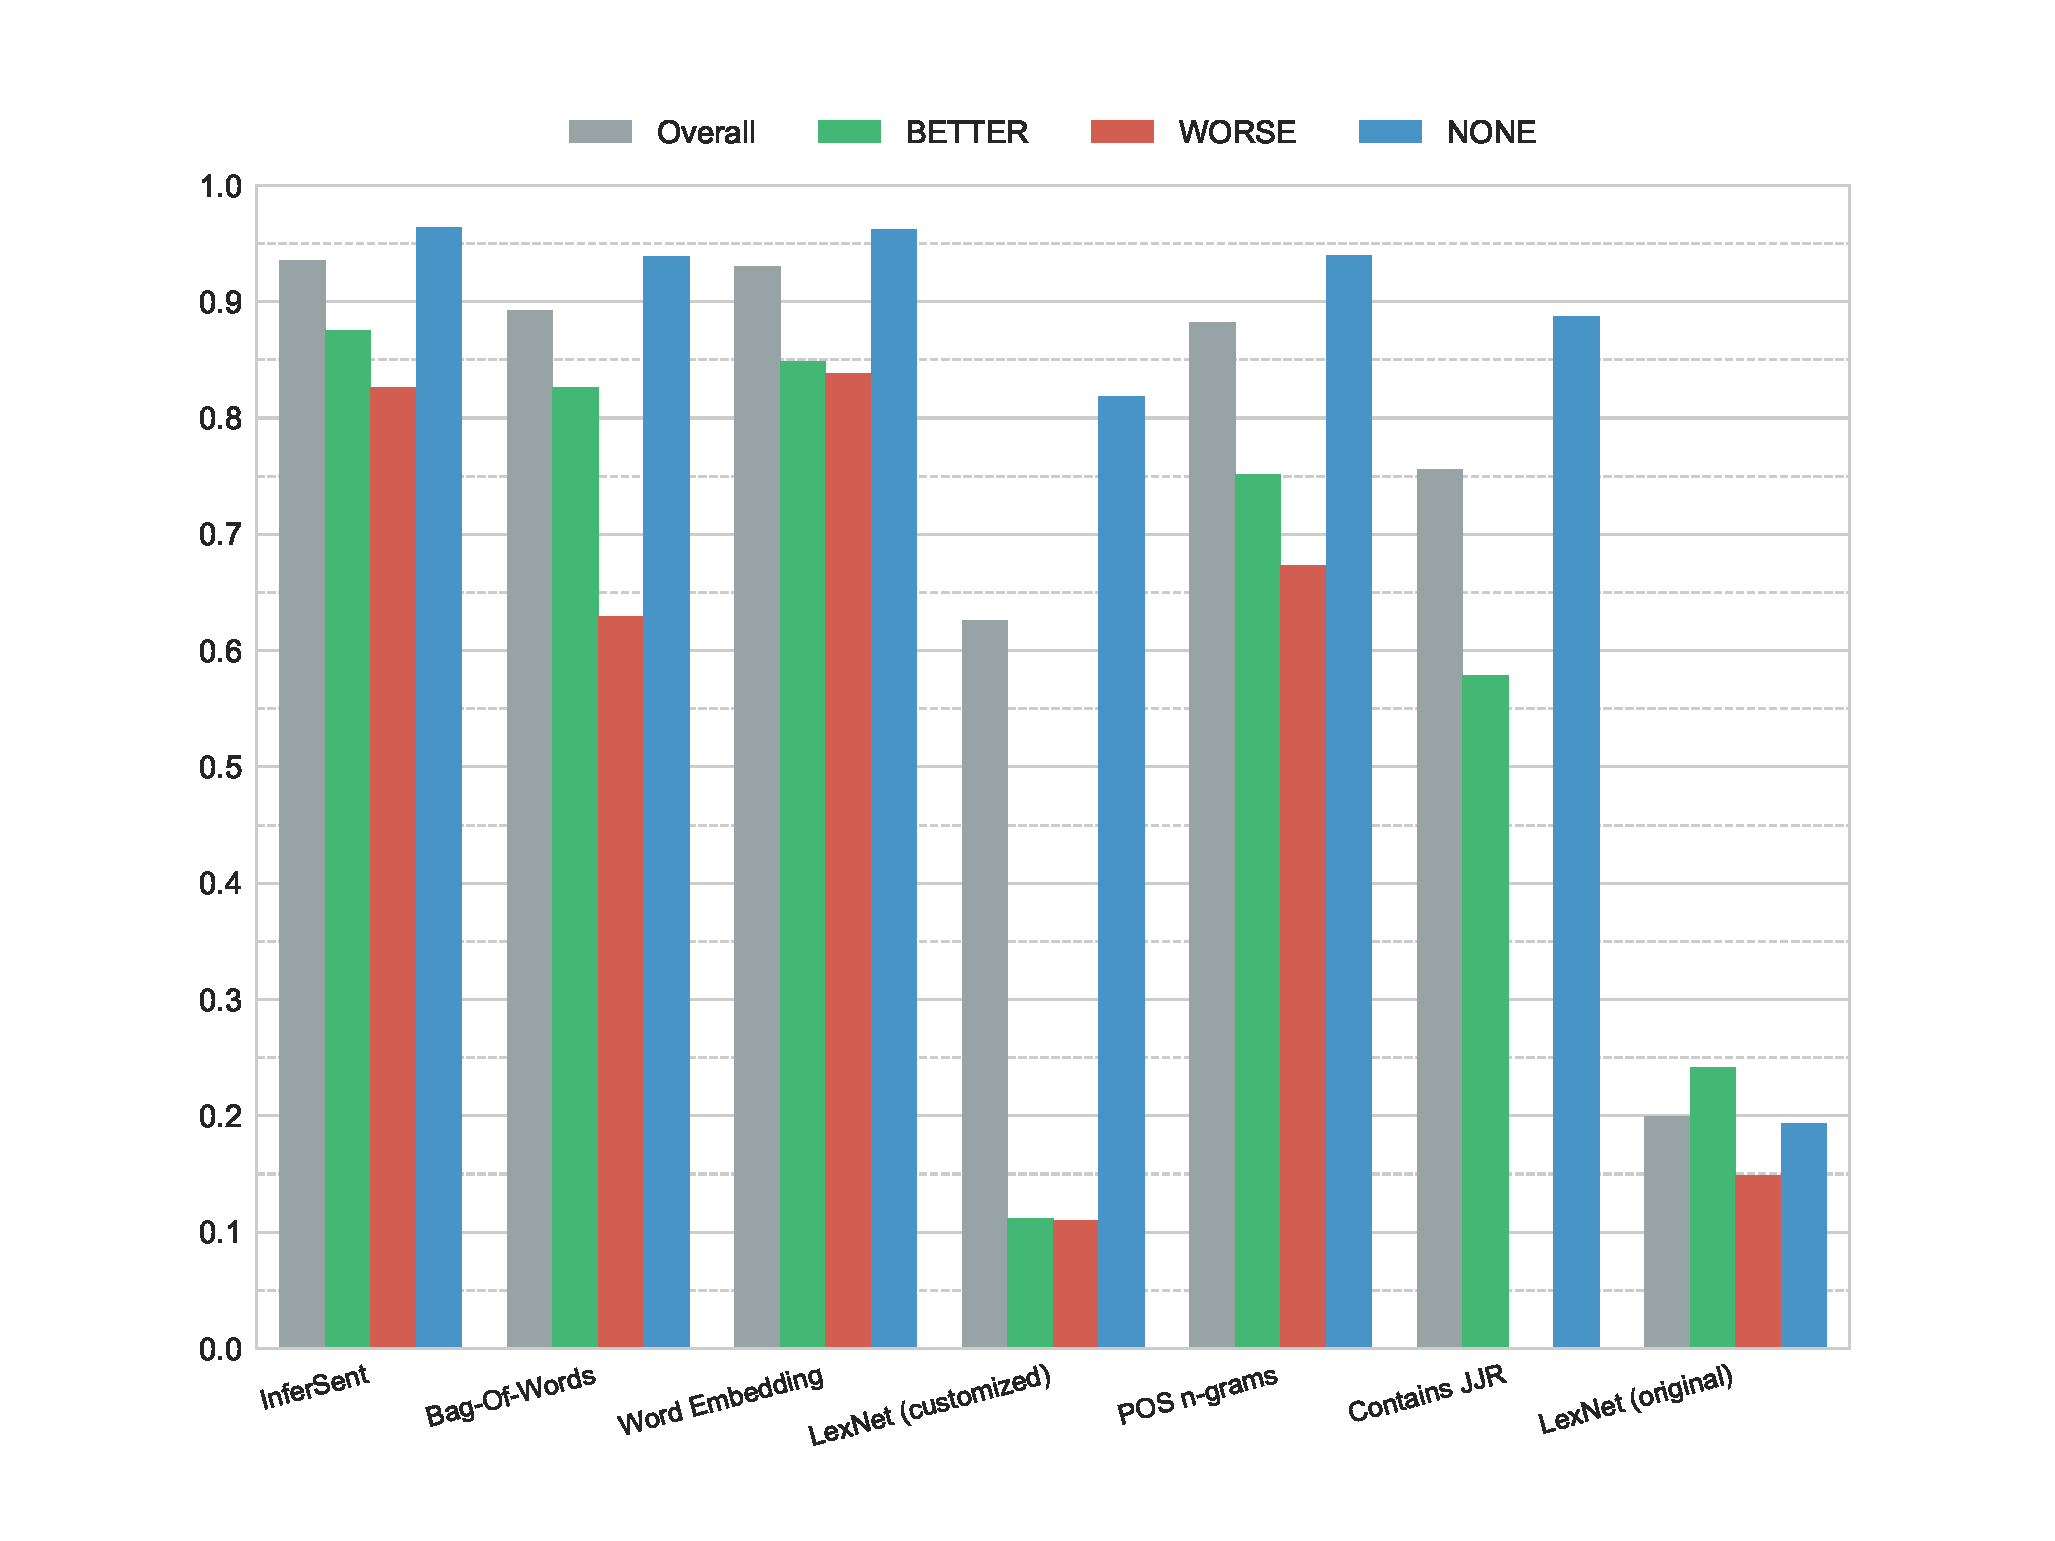
\includegraphics[width=1\linewidth]{images/heldout/h-f1-False}
    \end{figure}
    


\begin{figure}[htbp]
         \caption{\textbf{Precision} for the three-class scenario using XGBoost with the held-out data. The grey bar shows the weighted average. The feature names (see Section \ref{sec:features}) is presented on the x-axis, the precision score on the y-axis.} 
    \label{fig:h_3_prec}
    \centering
	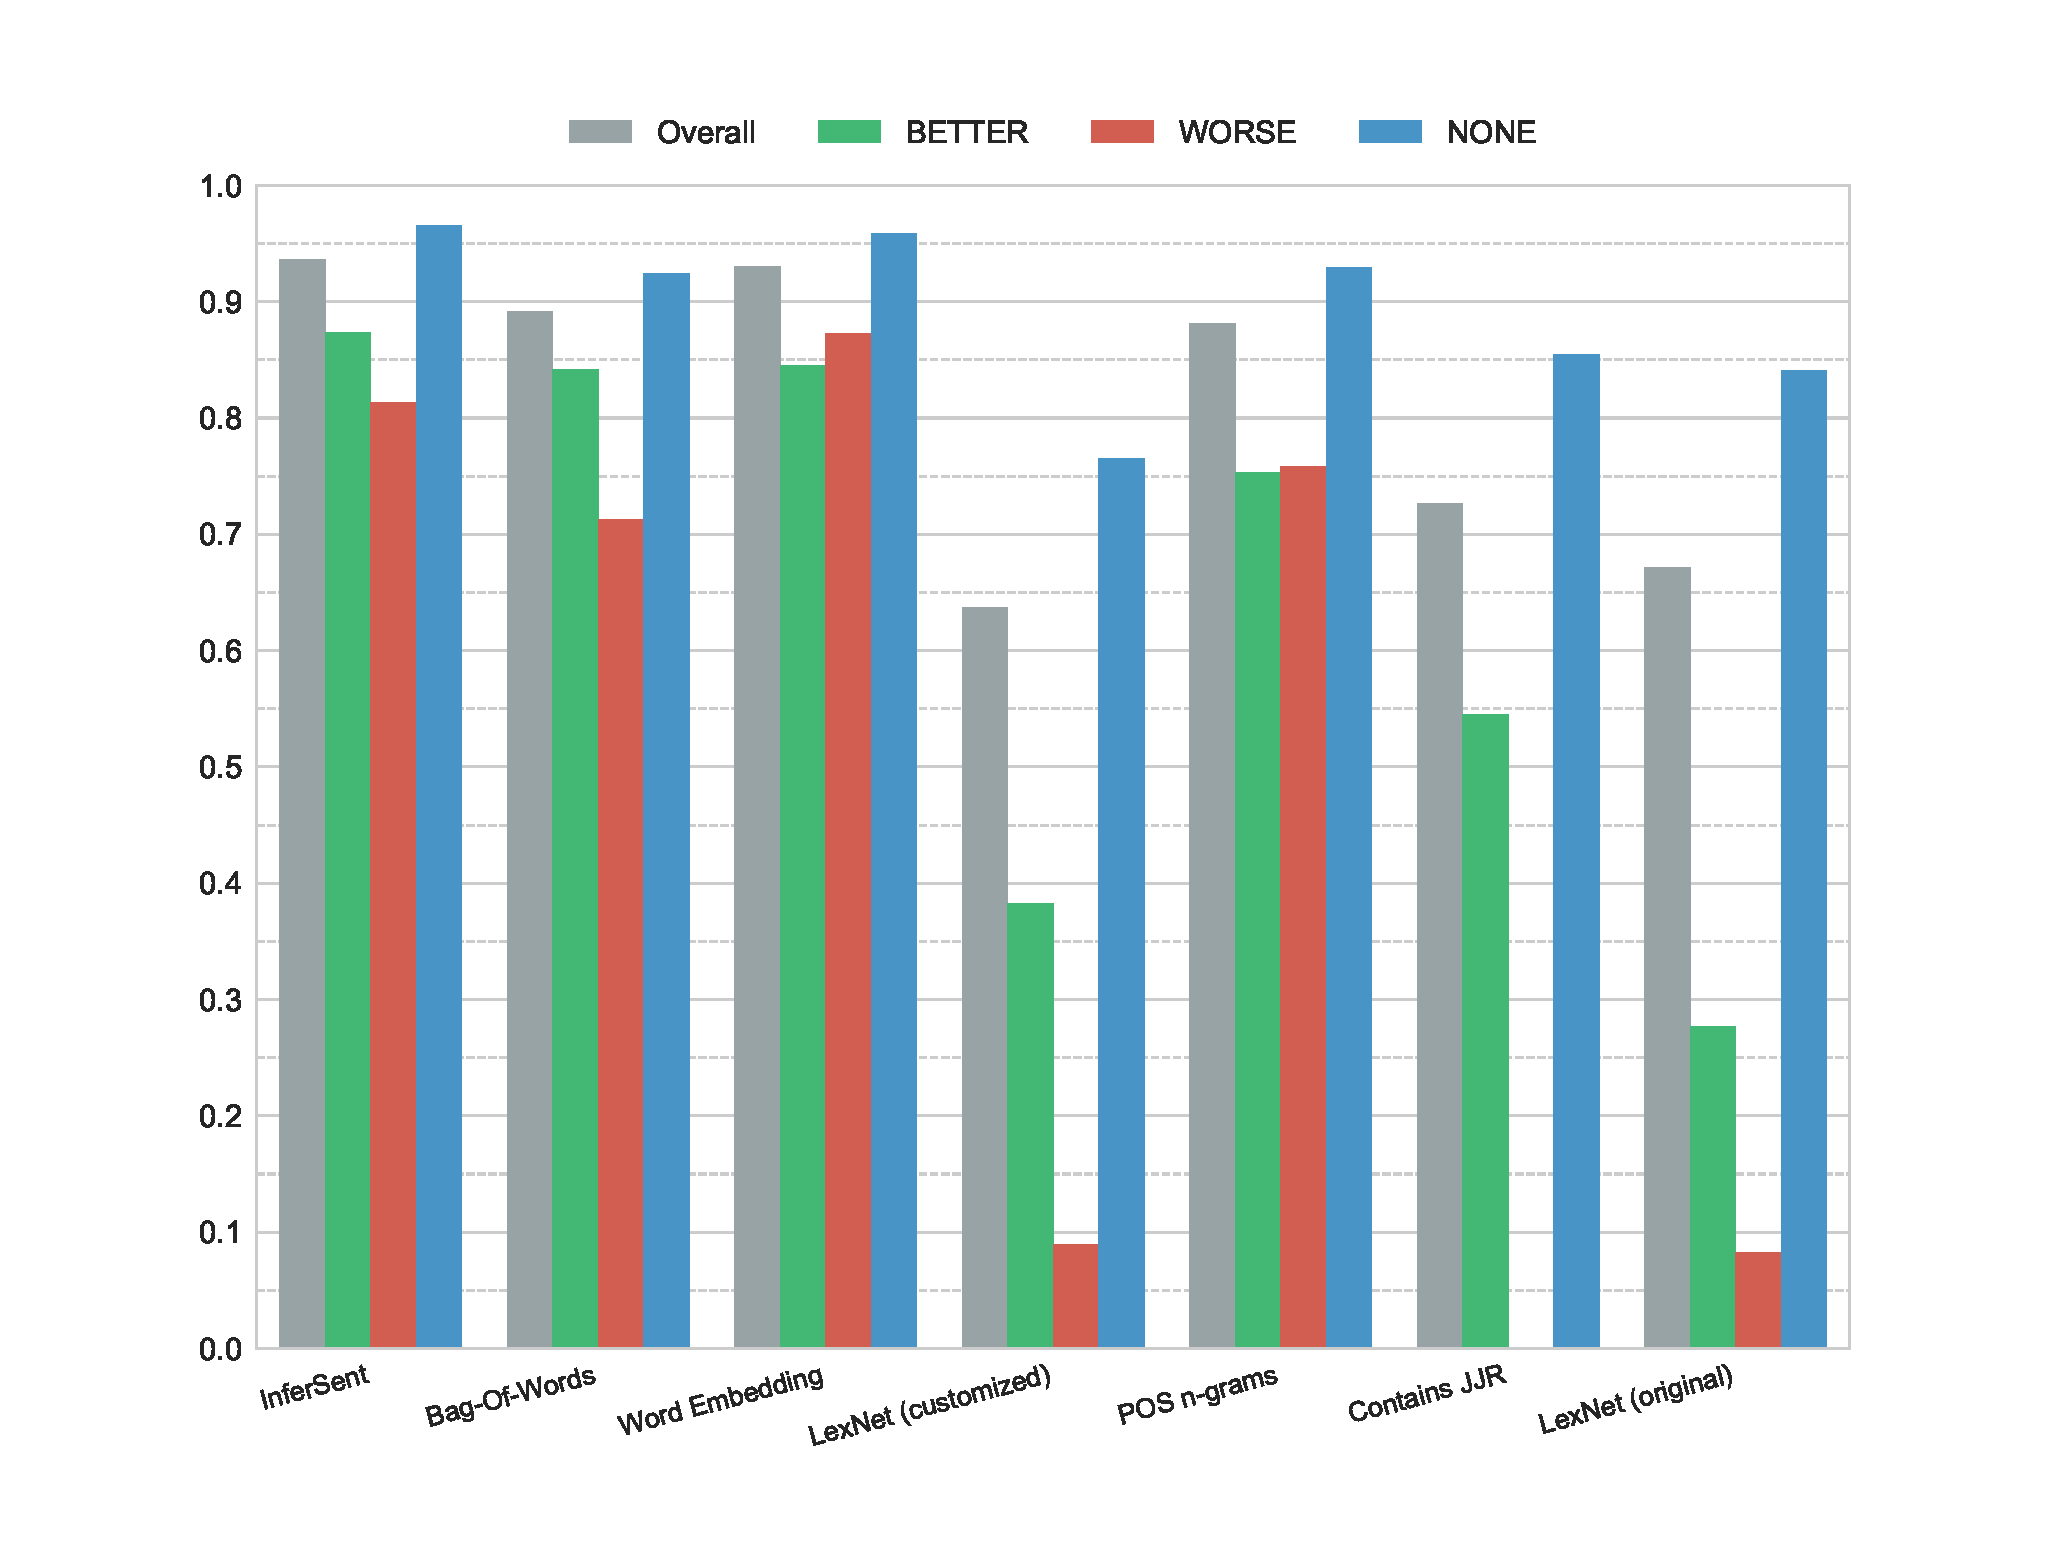
\includegraphics[width=0.9\linewidth]{images/heldout/h-precision-False}
    \end{figure}
    
    \begin{figure}[htbp]
              \caption{\textbf{Recall} for the three-class scenario using XGBoost with the held-out data. The grey bar shows the weighted average. The feature names (see Section \ref{sec:features}) are presented on the x-axis, the recall score on the y-axis.} 
       \label{fig:h_3_rec}
 \centering
	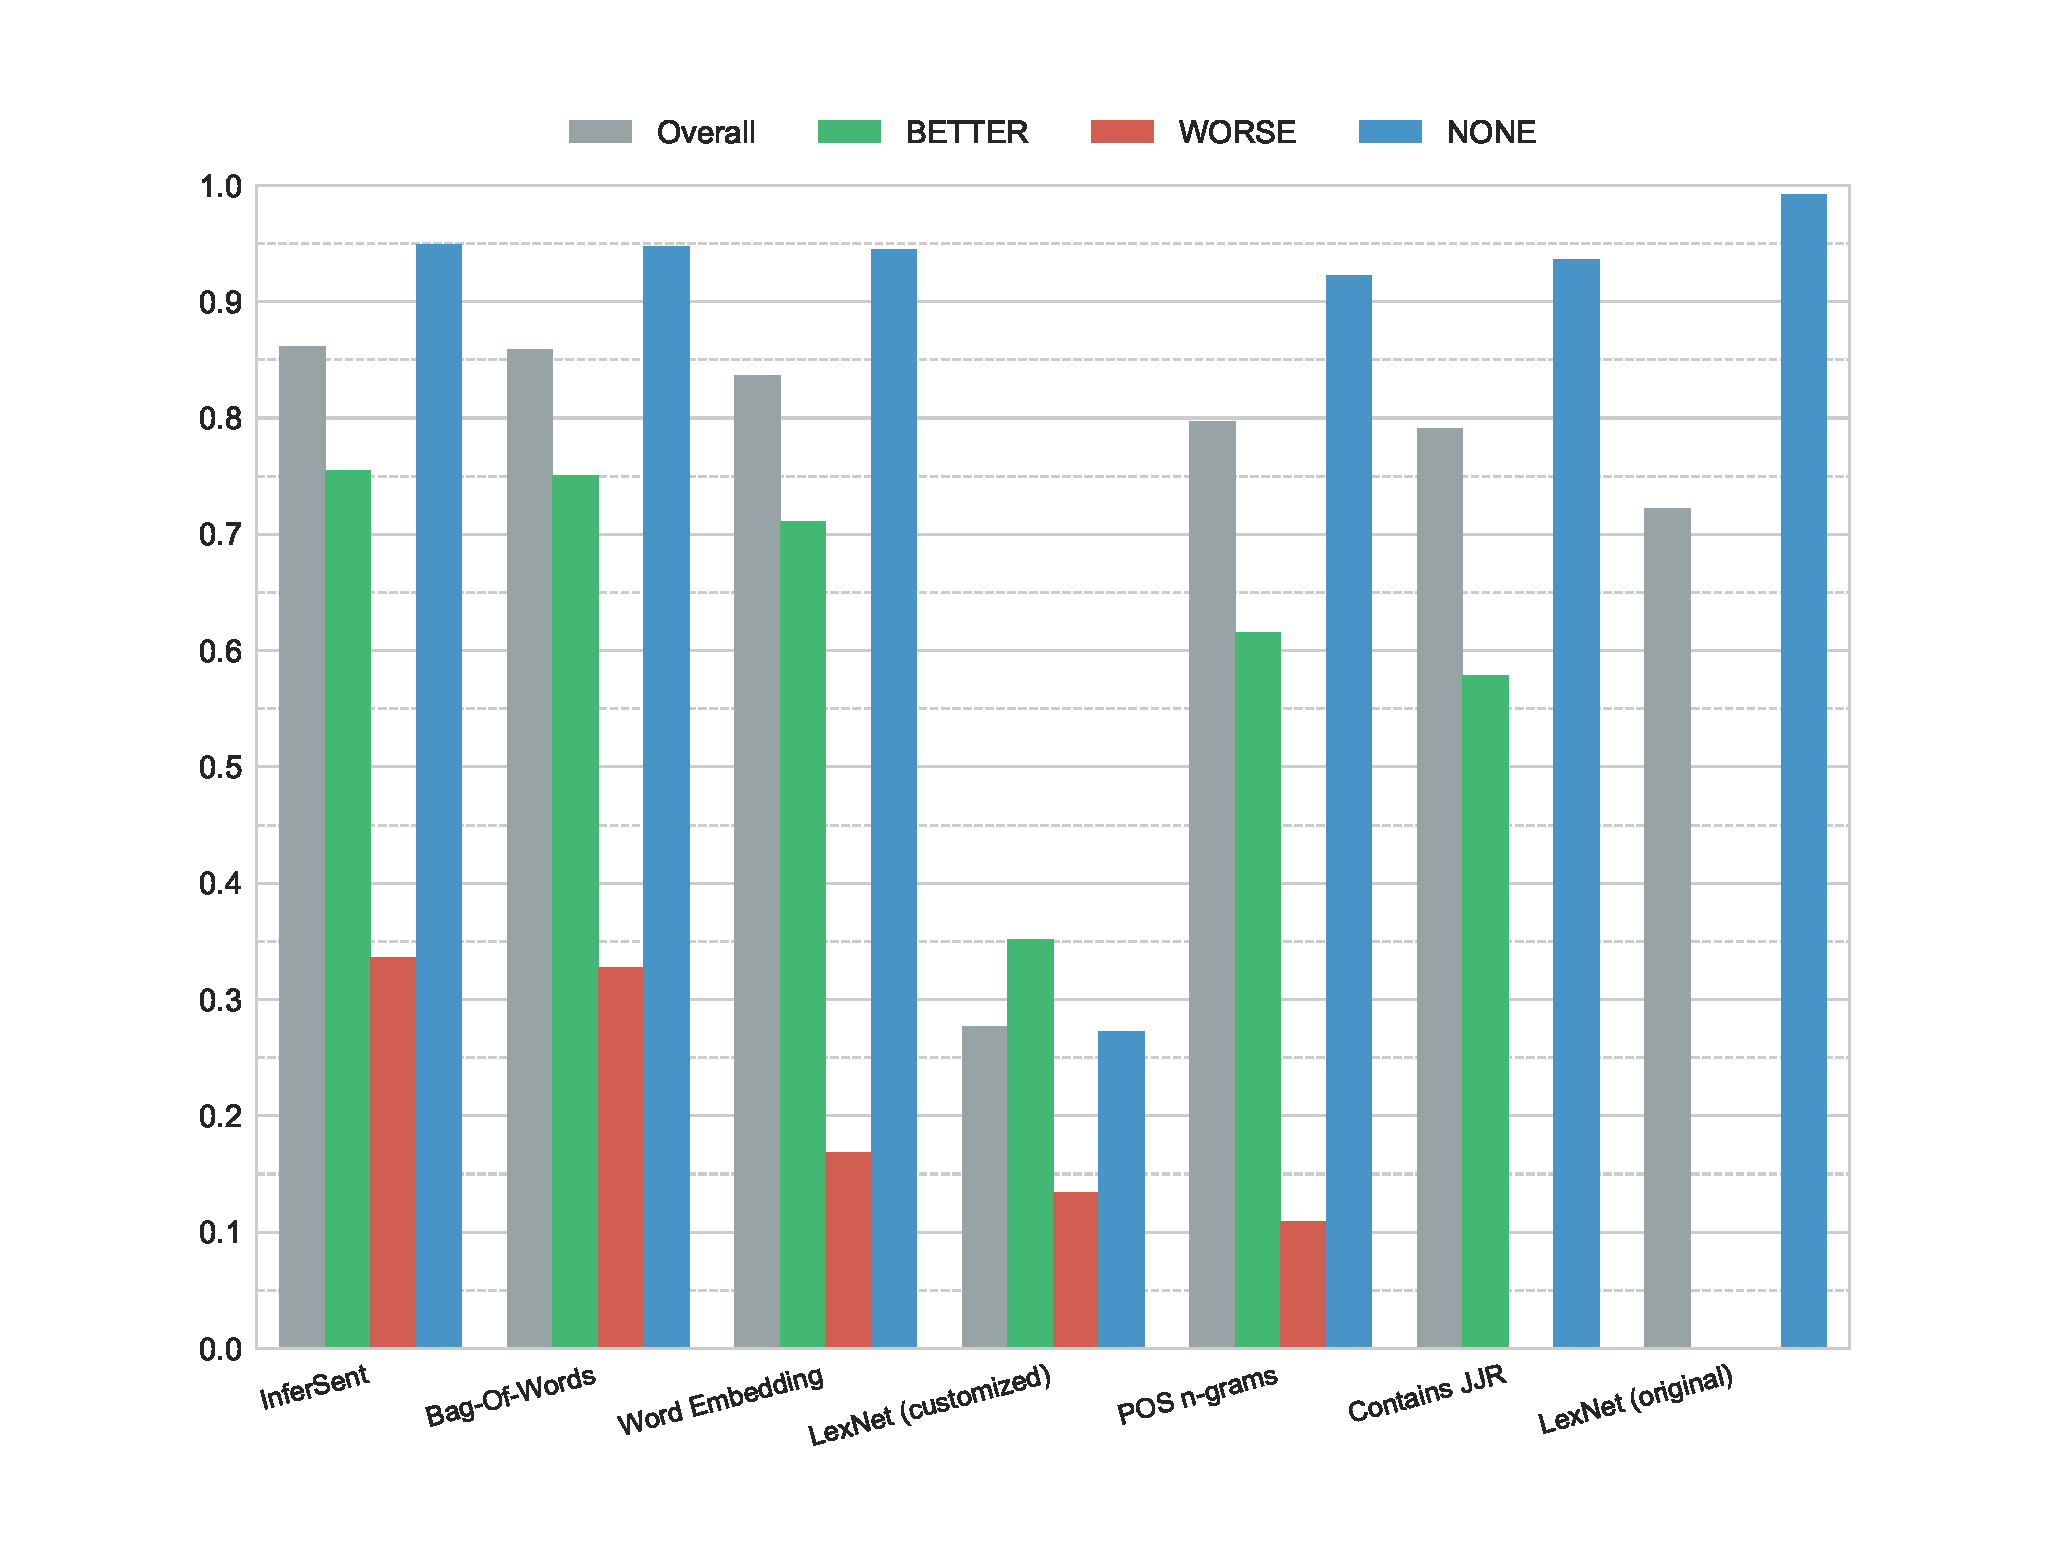
\includegraphics[width=0.9\linewidth]{images/heldout/h-recall-False}

\end{figure}

\FloatBarrier

The results for the binary scenario are presented in Figure \ref{fig:h_2_f1} (f1 score), Figure \ref{fig:h_2_prec} (precision) and Figure \ref{fig:h_2_rec} (recall).

% BINARY
\begin{figure}[htbp]
         \caption{\textbf{F1 score} for the binary scenario using XGBoost with the held-out data. The grey bar shows the weighted average. The feature names (see Section \ref{sec:features}) are presented on the x-axis, the f1 score on the y-axis.} 
    \label{fig:h_2_f1}
    \centering
	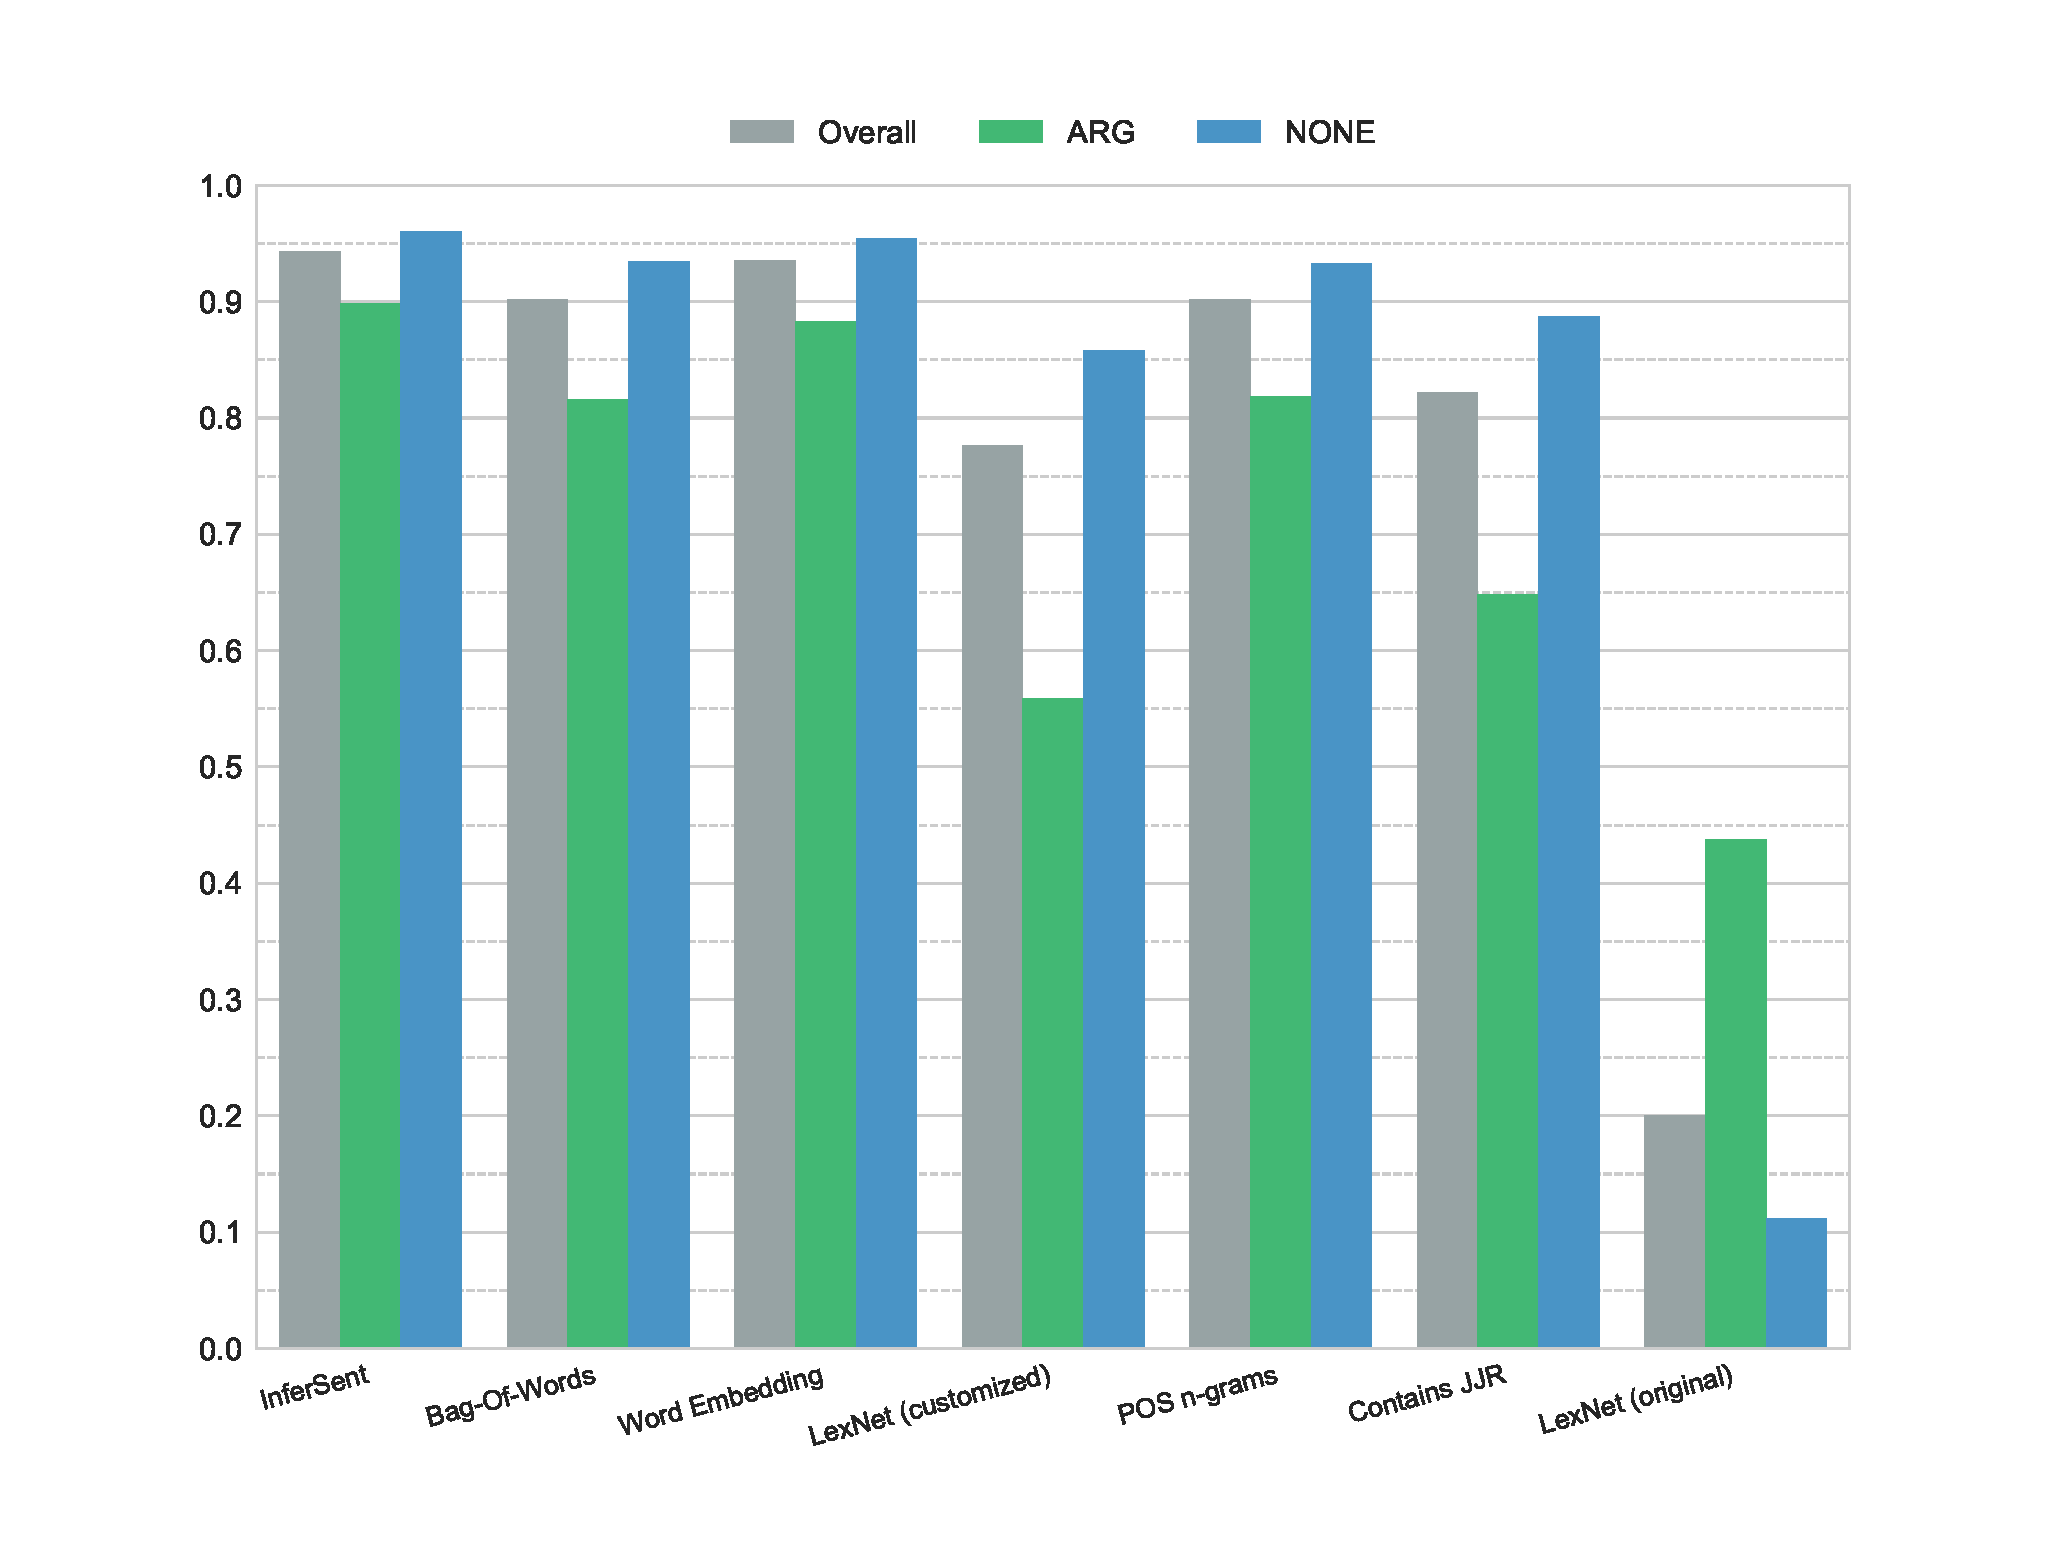
\includegraphics[width=0.9\linewidth]{images/heldout/h-f1-True}
    \end{figure}


\begin{figure}[htbp]
         \caption{\textbf{Precision} for the binary scenario using XGBoost with the held-out data. The grey bar shows the weighted average. The feature name (see Section \ref{sec:features}) are presented on the x-axis, the precision score on the y-axis.} 
    \label{fig:h_2_prec}
    \centering
	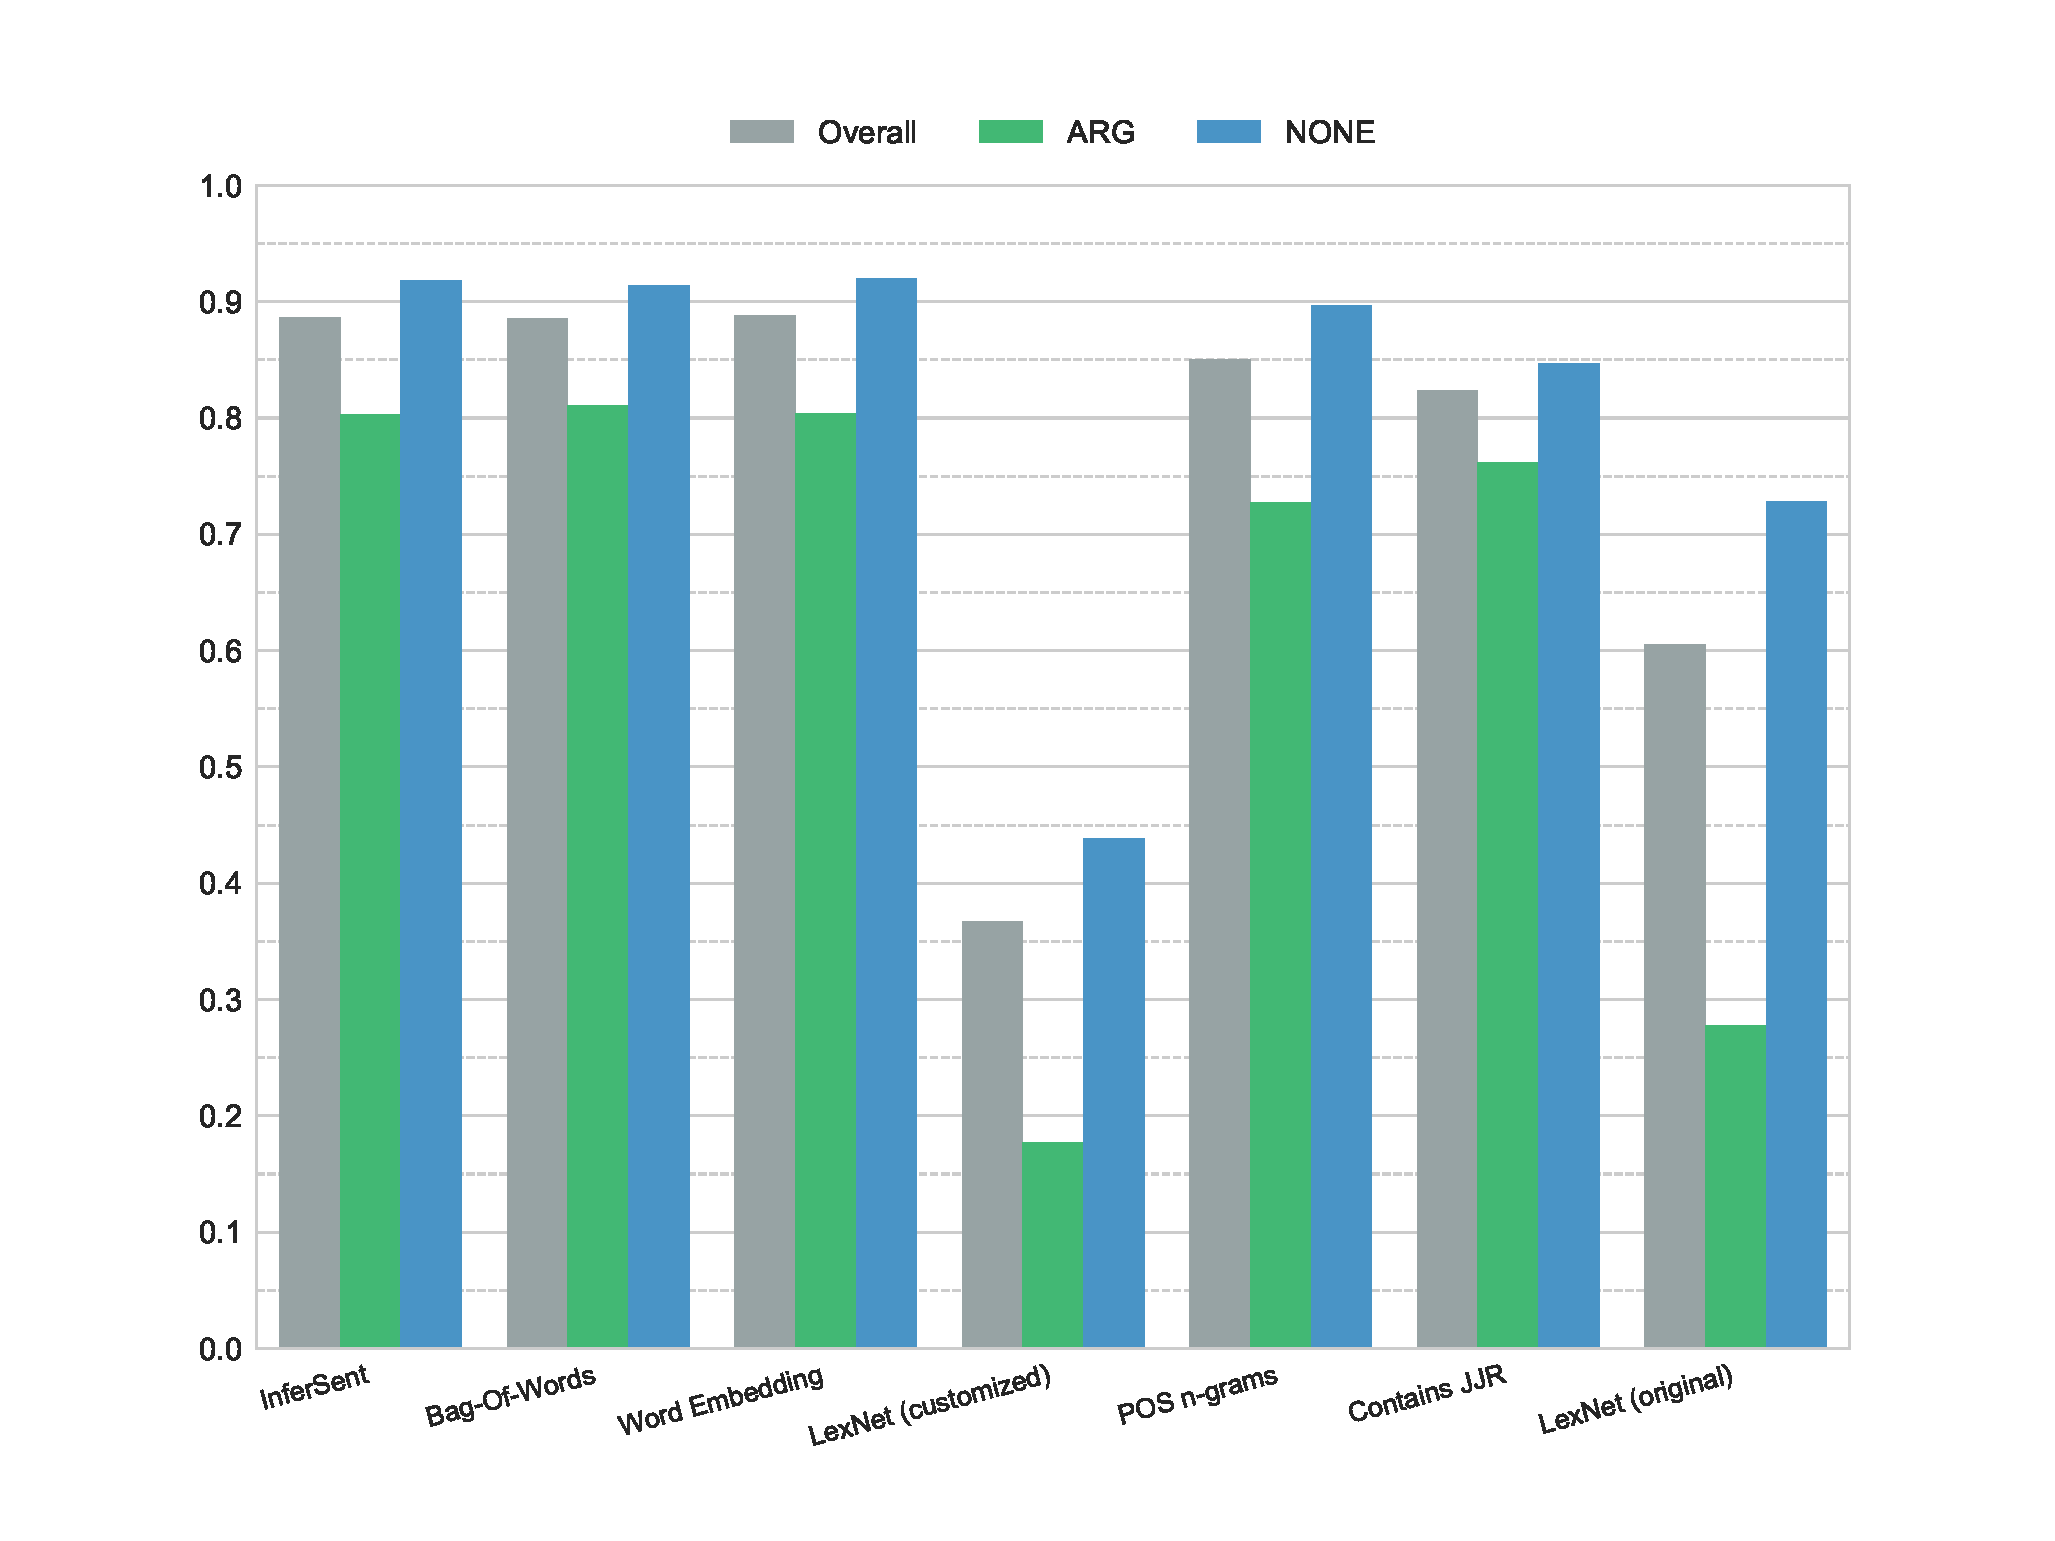
\includegraphics[width=0.9\linewidth]{images/heldout/h-precision-True}
    \end{figure}
    
    \begin{figure}[htbp]
              \caption{\textbf{Recall} for the binary scenario using XGBoost with the held-out data. The grey bar shows the weighted average. The feature names (see Section \ref{sec:features}) are presented on the x-axis, the recall score on the y-axis.} 
       \label{fig:h_2_rec}
 \centering
	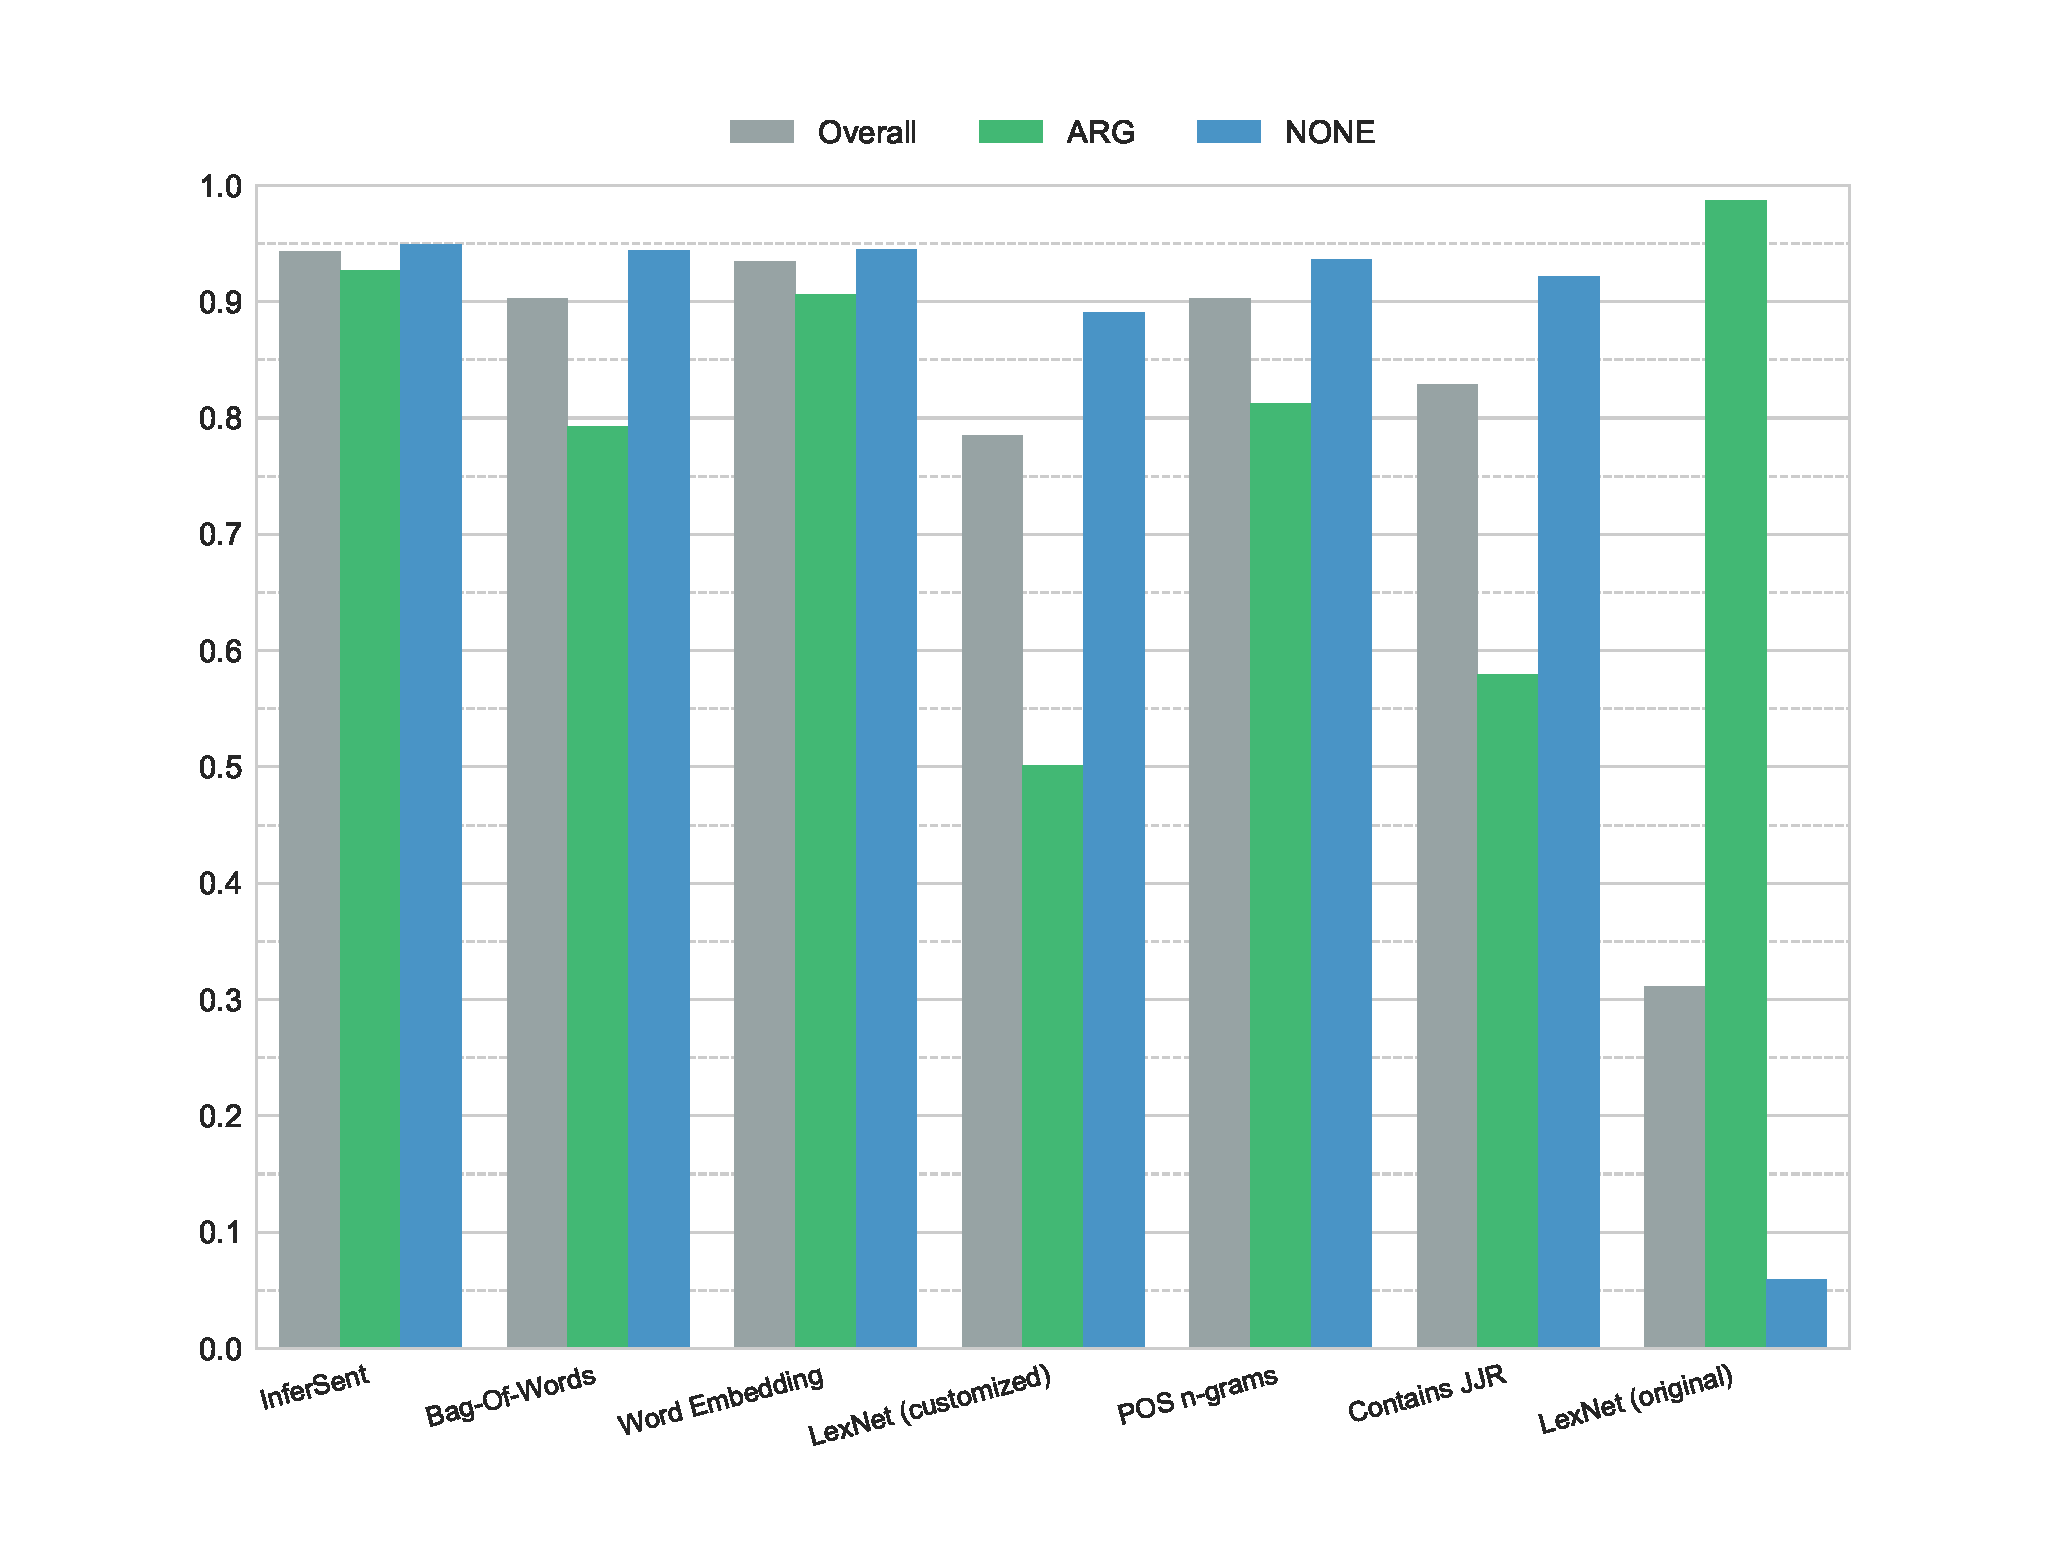
\includegraphics[width=0.9\linewidth]{images/heldout/h-recall-True}

\end{figure}
\FloatBarrier
\subsection{Discussion}
All features except LexNet benefited from the increased size of the training data, yet the increase of the f1 score is not larger than one or two points.\newline

LexNet did not generalise at all. The original setup predictsed \texttt{NONE} to all examples in the three-class scenario, thus it got the same f1 score as the baseline. It was able to predicts a small portion to \texttt{ARG} in the binary scenario, so that the f1 score was one point above the baseline. The customised version predicted all classes, yet the results were 27 points below the baseline for the three-class scenario and 38 points below in the binary scenario.

The problem was the size of the data set. LexNet created 2344 unique paths for the 5759 examples in the training data and 593 unique paths for the 1441 examples in the held-out data. As a result, one path only represented few sentences. Training and held-out had only 81 paths in common. The same is true for the customised setup, were even more paths were created (4339 for the training data and 1263 for the held-out data). Training and held-out only shared 228 paths. So, from LexNets point of view, training and held-out data are highly dissimilar.

This problem can be reduced with a larger data set. The Wikipedia corpus used in \cite{DBLP:conf/acl/ShwartzGD16} is magnitudes larger: it contains 4,682,000 articles.\footnote{Wikipedia Dump from 2015, \url{https://en.wikipedia.org/wiki/Wikipedia:Size_of_Wikipedia} (checked 15.5.2018)} The ratio between paths and sentences are much smaller in a corpus of this size.

The results with the training data alone (Section \ref{sec:3_results}) can be explained by the fact that the paths of all training examples were learned simultaneously. In contrast, the held-out embeddings were learned without information from the training set. The performance of the LexNet feature increases if the path embeddings are learned on the whole data (training and held-out; see figures \ref{fig:jl_3_f1} and  \ref{fig:jl_2_f1}).


\begin{figure}[htbp]
         \caption{\textbf{F1 score} for the LexNet feature in the three-class scenario. This time, path embeddings were learned on all sentences (training and held-out). XGBoost was trained on the training data and tested on the held-out data.} 
    \label{fig:jl_3_f1}
    \centering
	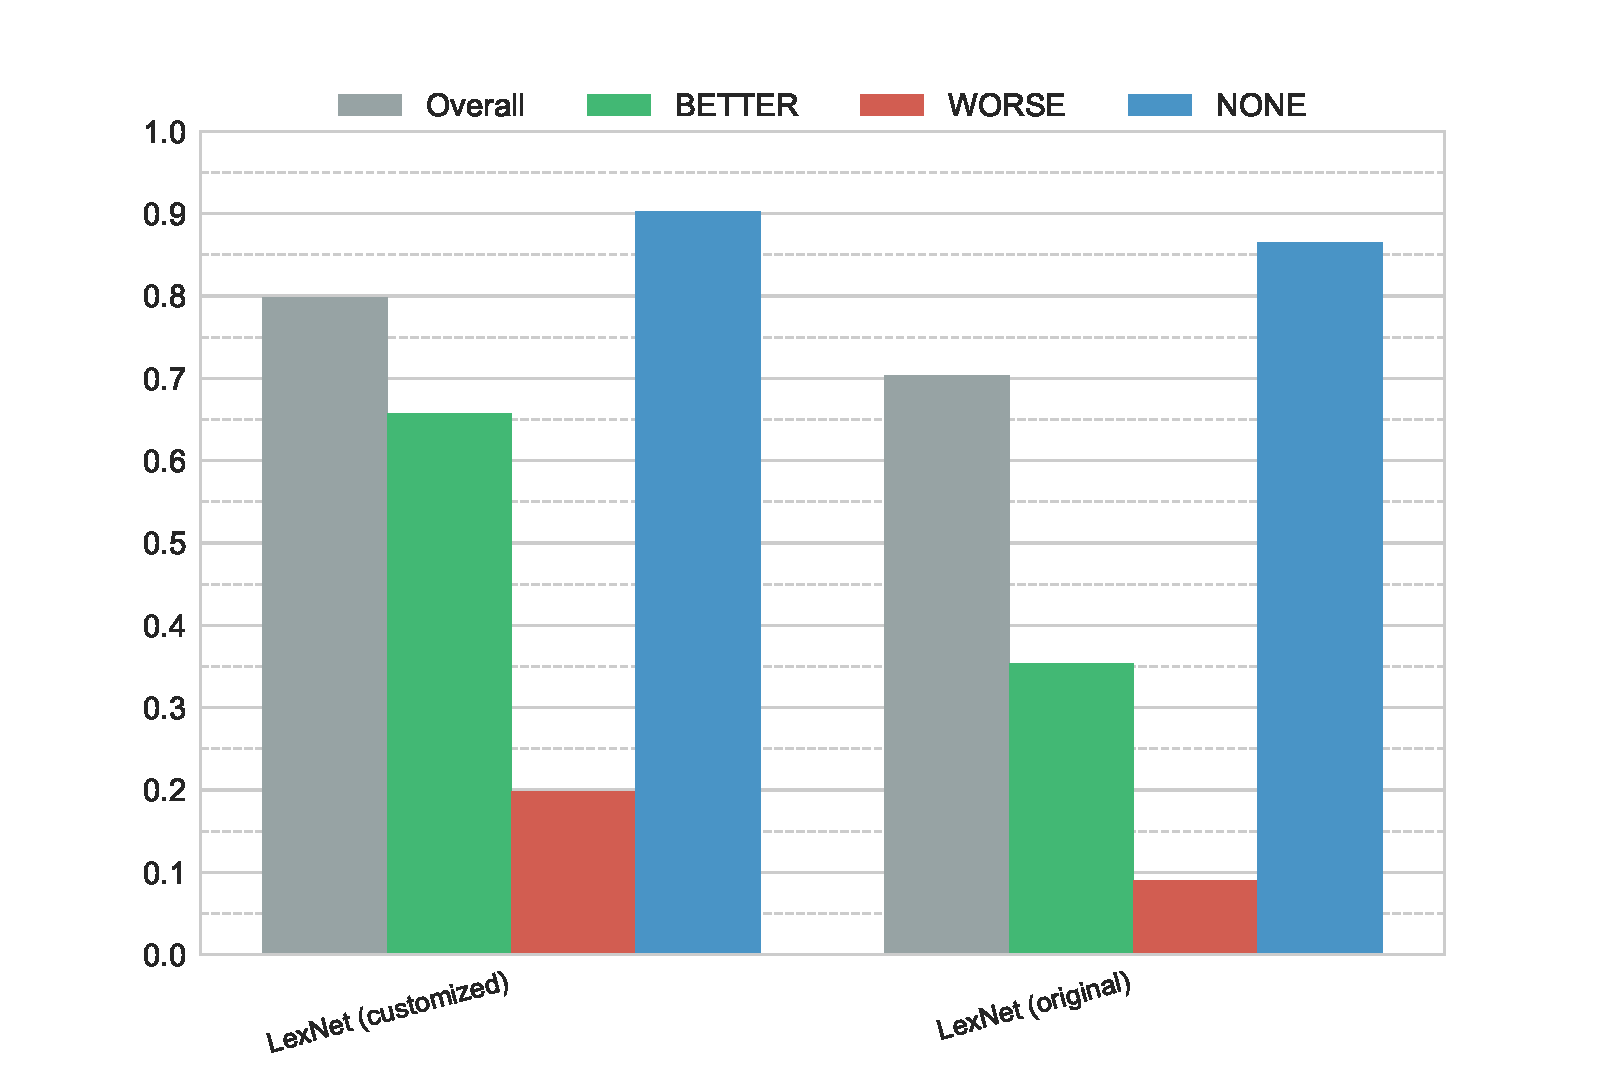
\includegraphics[width=1\linewidth]{images/extra/jl-f1-False}
    \end{figure}
    
    
\begin{figure}[htbp]
         \caption{\textbf{F1 score} for the LexNet feature in the binary scenario. This time, path embeddings were learned on all sentences (training and held-out). XGBoost was trained on the training data and tested on the held-out data.} 
    \label{fig:jl_2_f1}
    \centering
	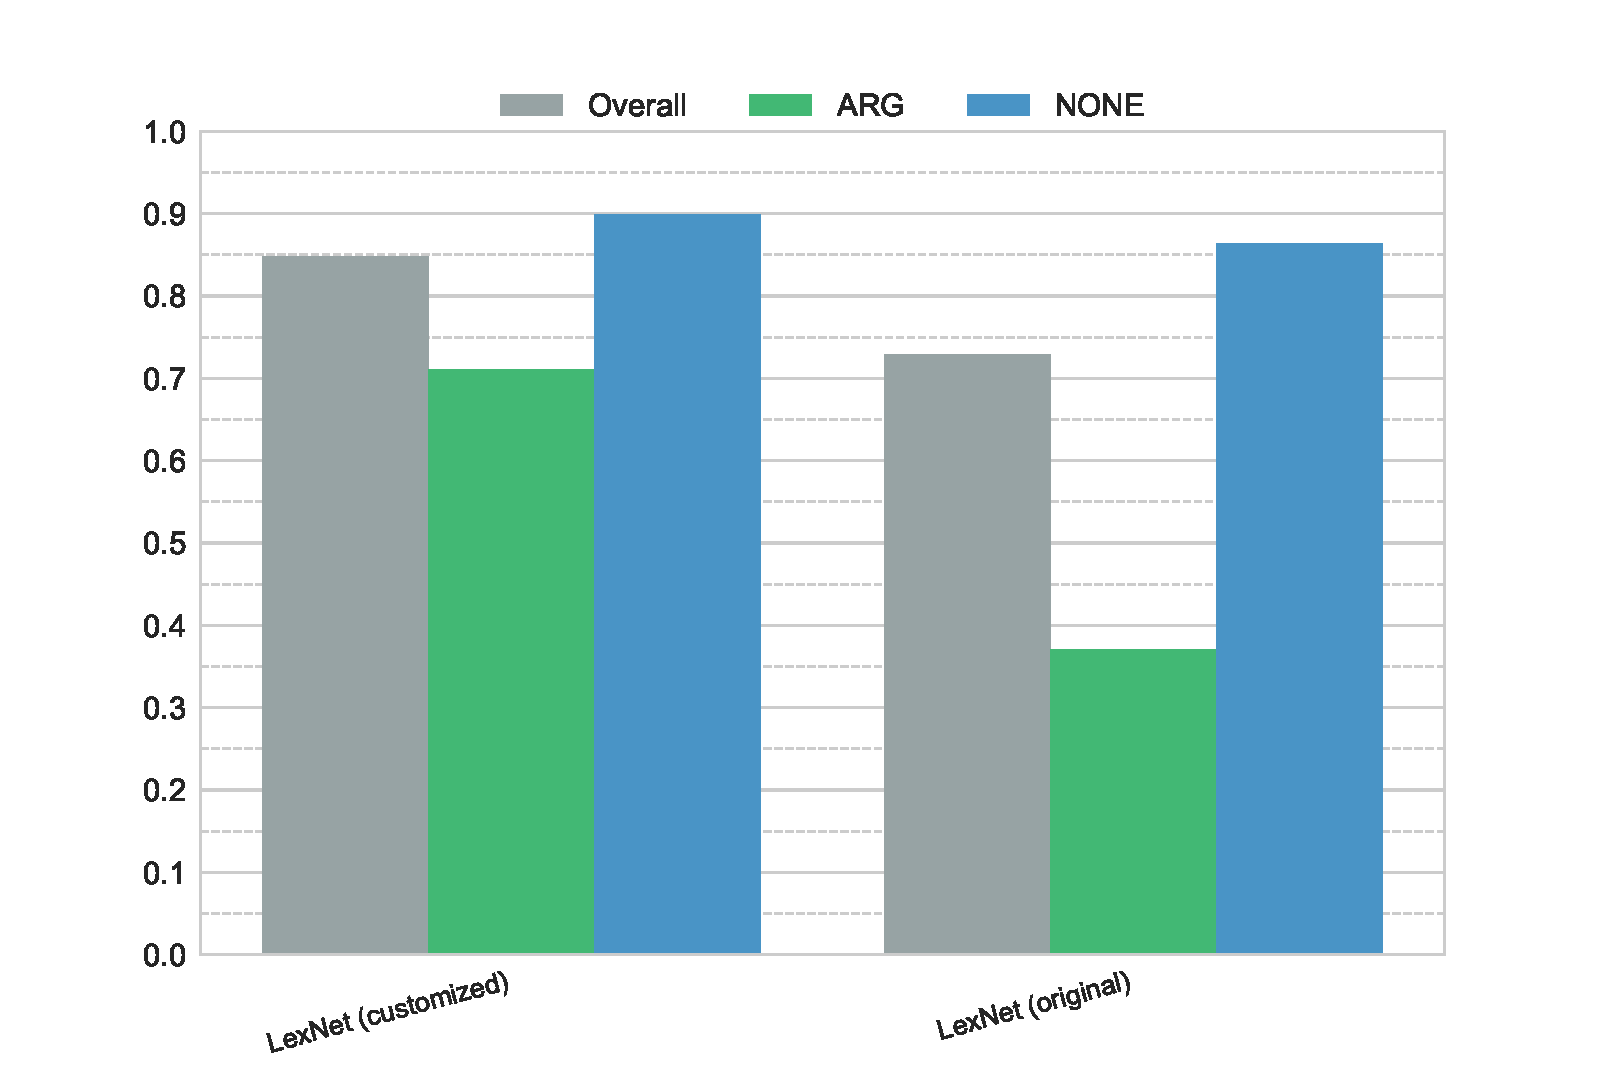
\includegraphics[width=1\linewidth]{images/extra/jl-f1-True}
    \end{figure}
